\documentclass[a4paper,11pt]{amsart}
\usepackage{geometry}
\geometry{a4paper,left=35mm,right=35mm, top = 35mm, bottom=35mm}

\usepackage[utf8]{inputenc}
\usepackage[T1]{fontenc}
\usepackage{setspace}
%\usepackage[ngerman]{babel}
\usepackage{lmodern}


\usepackage{amsmath}
\usepackage{amsthm}
\usepackage{amssymb}
% Boldface Zahlen
\usepackage{bbm}
\usepackage{enumerate}
\usepackage{mathtools}

%For include without pagebreak
\usepackage{newclude}

% For relative Textsizes
\usepackage{relsize}

%For units
\usepackage[binary-units=true]{siunitx}

\usepackage[disable]{todonotes}

\usepackage{graphicx}
% Bibliographi
%\usepackage{natbib}

%Für Quellcode
\usepackage{listings}

%Für Verlinkungen im Dokument
\usepackage{xcolor}
\definecolor{white}{rgb}{1,1,1}
\usepackage[linkbordercolor=white,urlbordercolor=white ,citebordercolor=white, plainpages=false]{hyperref}

%Zum Erstellen von Graphen für Automaten
\usepackage{tikz}
\usetikzlibrary{arrows,shapes.geometric,automata,positioning}
\tikzset{elliptic state/.style={draw,ellipse}}

%Diagrams
\usepackage[arrow, matrix, curve]{xy}


%For extra small fraction \sfrac 
\usepackage{xfrac}

%Reset the equation counter after each subsection
\usepackage{chngcntr}
\counterwithin*{equation}{section}
\counterwithin*{equation}{subsection}
%Für Zeilennummern
%\usepackage[modulo]{lineno}
%\linenumbers

%Counter für Automaten
\newcounter{automatonnumber}[section]
\renewcommand{\theautomatonnumber}{\mathcal{A}_{\thesection,\arabic{automatonnumber}}}
\newcommand{\autno}[1]{
  \refstepcounter{automatonnumber}
  \label{#1}
  (\theautomatonnumber)
}

%Quellcode Aussehen:
\lstset {
basicstyle=\normalsize,
language=GAP,
breaklines=true,
showstringspaces=false,
tabsize=2
}
%Monospace in inline code
%\lstMakeShortInline[columns=fixed]|

\newtheorem{pro}{Proposition}[section]
\newtheorem{con}[pro]{Conjecture}
\newtheorem{thm}[pro]{Theorem}
\newtheorem{cor}[pro]{Corollary}
\newtheorem{lem}[pro]{Lemma}

\newtheorem{task}{Task}

\theoremstyle{definition}
\newtheorem*{ex}{Example}
\newtheorem*{re}{Remark}
\newtheorem{defi}[pro]{Definition}
\newtheorem{cordef}[pro]{Corolary/Definition}


%Für Quotienten
\newcommand{\RRNK}[2]{
  \raisebox{1ex}{\ensuremath{#1}}
  \ensuremath{\mkern-3mu} \bigg/  \ensuremath{\mkern-3mu}
  \raisebox{-1ex}{\ensuremath{#2}}
}
\newcommand{\RNK}[2]{{#1/#2}}
% \newcommand{\RNK}[2]{
%   \mathchoice{ \raisebox{1ex}{\ensuremath{#1}}%
% 	       \ensuremath{\mkern-4mu} \big/  \ensuremath{\mkern-4mu}%
% 	       \raisebox{-1ex}{\ensuremath{#2}}}%
% 	     { \raisebox{0.2ex}{\ensuremath{#1}}%
% 	       \ensuremath{\mkern-4mu} /  \ensuremath{\mkern-4mu}%
% 	       \raisebox{-0.2ex}{\ensuremath{#2}}}%
% 	     { \raisebox{0.1ex}{\ensuremath{\scriptstyle#1}}%
% 	       \ensuremath{\mkern-4mu} /  \ensuremath{\mkern-4mu}%
% 	       \raisebox{-0.1ex}{\ensuremath{\scriptstyle#2}}}%
% 	     { {\ensuremath{#1}}%
% 	        /%
% 	       {\ensuremath{#2}}}%
%   \ 
% }

%uppergausian bracket
\DeclarePairedDelimiter{\ceil}{\lceil}{\rceil}

%Pfeile für exakte Sequenzen
\newcommand{\exar}[1][ ]{\overset{#1}{\longrightarrow}}
%Normalteiler/Ideal 
\newcommand{\normal}{{\mathrel\trianglelefteq}}

%großer Strich
\newcommand{\bigmid}{\ \middle \vert }

%Besondere Buchstaben
\newcommand{\NN}{\mathbb{N}}
\newcommand{\ZZ}{\mathbb{Z}}
\newcommand{\QQ}{\mathbb{Q}}
\newcommand{\RR}{\mathbb{R}}
\newcommand{\CC}{\mathbb{C}}
\newcommand{\HH}{\mathbb{H}}
\newcommand{\PP}{\mathbb{P}}
\newcommand{\one}{\mathbbm{1}}

%das d hinter dem Integral
\newcommand{\intd}{d}

%Sprachen
\newcommand{\La}{\mathcal{L}}
\newcommand{\emptyword}{\epsilon}
%Zustandmenge
\newcommand{\States}{\zeta}
%Alphabet
\newcommand{\Al}{\mathcal{A}}
%Zentrum
\newcommand{\Ce}{\mathfrak{C}}
%Free Variables in a groupword
\newcommand{\Var}{\textup{Var}}
%Commutator width
\newcommand{\cw}{\textup{width}}
%Stabilizer
\newcommand{\Sta}{\textup{St}}
%Projektion auf Alphabet
\newcommand{\alphab}{\mathfrak{wr}}
\newcommand{\state}{\mathfrak{state}} 
%zugehörige Mealy
\newcommand{\mealy}[1]{\mathfrak{M}_{#1}}
%Aktivität eines Automorphismus
%\newcommand{\act}{\mathcal{A}\mathcal{CT}}
%\newcommand{\act}{{\scalebox{0.9}{$\mathcal{A}$}\mspace{-2mu}\raisebox{-0.3ex}{\tiny$\mathbf{ct}$}}}
\newcommand{\act}{{\textup{\smaller$\mathcal{A}\mathbf{ct}$}}}
%PairKlammern
\DeclarePairedDelimiter{\pair}{\langle\negthickspace\langle}{\rangle\negthickspace\rangle}
%\newcommand{\pair}[1]{{\langle\negthickspace\langle #1 \rangle\negthickspace\rangle}}
%Nucleus
\newcommand{\Nuc}{\mathcal{N}}
%Commutatror Width
\newcommand{\mcount}{{\#_M}}
%Normal normal_form
\newcommand{\nf}{\mathfrak{nf}}
%Reduced constraints
\newcommand{\Red}{\mathfrak{R}}
%Ideale
\newcommand{\ai}{\mathfrak{a}}
\newcommand{\bi}{\mathfrak{b}}
\newcommand{\Ji}{\mathcal{Ji}}

%Zustände von Automaten

%\newcommand{\at}[1]{  {\raisebox{-0.3ex}[1ex]{$\mathbin{@}$}#1} }
\newcommand{\at}[1]{  {{\textup{\smaller @}}#1} }
\newcommand{\att}[1]{  {{\bar{\textup{\smaller @}}}#1} }
%\newcommand{\at}[1]{  |_{#1} }

%Centralizer:
\newcommand{\centra}{\mathcal{C}}
%Stabilizer
\newcommand{\Stab}{\textup{Stab}}
%Undefined elememts
\newcommand{\undef}{\varnothing}

%Funktionen aufrecht
\newcommand{\Aut}{\textup{Aut}}
\newcommand{\RAut}{\textup{RAut}}
\newcommand{\FAut}{\textup{FAut}}
\newcommand{\Poly}{\textup{Poly}}
\newcommand{\EPoly}{\mbox{\smaller$\frac{1}{2}$}\Poly}
%\newcommand{\EPoly}{\textup{EPoly}}
\newcommand{\Orb}{\textup{Orb}}
\newcommand{\OS}{\textup{OS}}
\newcommand{\OSA}{\textup{OSA}}
\newcommand{\supp}{\textup{supp}}
\newcommand{\End}{\textup{End}}
\newcommand{\rad}{\textup{rad}}
\newcommand{\ad}{\textup{ad}}
\newcommand{\id}{\mathbbm{1}}
\newcommand{\im}{\textup{i}}
\newcommand{\Min}{\textup{Min}}
\newcommand{\Imm}{\textup{Im}}
\newcommand{\Span}{\textup{span}}
\newcommand{\Spec}{\textup{Spec}}
\newcommand{\Spur}{\textup{tr}}
\newcommand{\rk}{\textup{rk}}
\newcommand{\sign}{\textup{sign}}
\newcommand{\diag}{\textup{diag}}
\newcommand{\Sym}{\textup{Sym}}
\newcommand{\ord}{\textup{ord}}
\newcommand{\suc}{\textup{suc}}
\DeclareMathOperator{\lcm}{lcm}
\DeclareMathOperator{\operp}{{ \bigcirc\!\!\!\!\!\!\!\perp}}

\newcommand{\BIGOP}[1]{\mathop{\mathchoice%
{\raise-0.22em\hbox{\huge $#1$}}%
{\raise-0.05em\hbox{\Large $#1$}}{\hbox{\large $#1$}}{#1}}}
\newcommand{\bigtimes}{\BIGOP{\times}}

\newcommand{\bigcomp}{\BIGOP{\circ}}

% nur fuer Bigboxplus andere Korrekturen
\newcommand{\BIGboxplus}{\mathop{\mathchoice%
{\raise-0.35em\hbox{\huge $\boxplus$}}%
{\raise-0.15em\hbox{\Large $\boxplus$}}{\hbox{\large $\boxplus$}}{\boxplus}}}
\parindent=0em

% For filenames
\newcommand{\filename}[1]{{\texttt{#1}}}
%TODO replace this by a nicer one
\newcommand{\gapinline}[1]{{\lstinline{#1}}}

\bibliographystyle{amsalpha}

\begin{document}
\title{Commutator width in the first Grigorchuk group}
\author{Laurent Bartholdi}
\author{Thorsten Groth}
\author{Igor Lysionok}
\begin{abstract}
  Let $G$ be the first Grigorchuk group.  We show that the commutator
  width of $G$ is $2$: every element $g\in [G,G]$ is a product of two
  commutators. Furthermore, we show that every finitely generated
  subgroup $H\leq G$ has finite commutator width, which however can be
  arbitrarily large. The proofs were assisted by the computer algebra
  system GAP.
\end{abstract}
\maketitle
%\tableofcontents

%%%%%%%%%%%%%%%%%%%%%%%%%%%%%%%%%%%%%%%%%%%%%%%%%%%%%%%%%%%%%%%%
\section{Introduction}
Let $\Gamma$ be a group and let $\Gamma'=[\Gamma,\Gamma]$ denote its
derived subgroup. The \emph{commutator width} of $\Gamma$ is the least
$n\in \NN\cup \infty$ such that every element of $\Gamma'$ is a
product of $n$ commutators.

We compute, in this article, the commutator width of the \emph{first
  Grigorchuk group} $G$. This is a prominent example from the class of
\emph{branched groups}, and as such is a good testing ground for
decision and algebraic problems in group theory. We prove:
\begin{thma}\label{thm:CWGrigorchukGroup}
  The first Grigorchuk group and its branching subgroup have
  commutator width $2$.
\end{thma}
It was already proven in~\cite{Lysenok-Miasnikov-Ushakov:QuadraticEquationsInGrig} that
the commutator width of $G$ is finite, with an inherently inexplicit
method. Our proof does not rely on that previous work. Our result also
answers a question of Elisabeth
Fink~\cite[Question~3]{Fink:Conjugacy_growth}:
\begin{cora}\label{cor:productOf6Conjugates}
  Every element of $G'$ is a product of $6$ conjugates of the
  generator $a$ and there are elements $g\in G'$ which are 
  not products of $4$ conjugates of $a$.
\end{cora}


There are examples of groups of finite commutator width with subgroups
of infinite commutator width; and even finitely presented, perfect
examples in which the subgroup has finite index. However, we can
prove:
\begin{thma}\label{thm:subgroups}
  Every finitely generated subgroup of $G$ has finite commutator
  width; however, their commutator width cannot be bounded, even among
  finite-index subgroups.
\end{thma}

\subsection{Commutator width}
Let $\Gamma$ be a group. It is well-known that sometimes elements of
$\Gamma'$ are not commutators---for example,
$[X_1,X_2]\cdots[X_{2n-1},X_{2n}]$ is not a commutator in the free
group $F_{2n}$. In fact, every non-abelian free group has infinite
commutator width, because it contains $F_{2n}$ for all $n$.

Finite groups, and more generally virtually abelian groups, have
finite commutator width.  There are finite groups in which some
elements are not commutators, the smallest having order $96$,
see~\cite{Guralnick:Group96}. On the other hand, non-abelian finite
simple groups have commutator width $1$, as conjectured by
Ore~\cite{Ore:Commutators} in~1951 and proven in~2010,
see~\cite{Liebeck:OreConjecture}. The commutator width cannot be
bounded among finite groups; for example,
$\Gamma=\langle x_1,\dots,x_{2n}\mid
x_1^p,\dots,x_{2n}^p,\gamma_3(\langle x_1,\dots,x_{2n})\rangle$ is a
finite class-$2$ nilpotent group in which $\Gamma'$ has order
$p^{\binom{2n}2}$ but at most $\binom{p^{2n}}2$ elements are
commutators.

Commutator width of groups, and of elements, has proven to be an
important group property, in particular via its connections with
``stable commutator length'' and bounded
cohomology~\cite{Calegari:SCL}. It is also related to solvability of
quadratic equations in groups: a group $\Gamma$ has commutator width
$\le n$ if and only if the equation
$[X_1,X_2]\cdots[X_{2n-1},X_{2n}]g=1$ is solvable for all
$g\in\Gamma$. Needless to say, there are groups in which solvability
of equations is undecidable. It was proven
in~\cite{Lysenok-Miasnikov-Ushakov:QuadraticEquationsInGrig} that quadratic equations are
solvable in the first Grigorchuk group $G$, and the mere existence of
an algorithm solving quadratic equations implies that $G$ has finite
commutator width, without giving an explicit bound.

We note that if the character table of a group $\Gamma$ is computable,
then it may be used to compute the commutator width: Burnside shows
(or, rather, hints) in~\cite[\S238, Ex. 7]{Burnside:Groups} that an
element $g\in\Gamma$ may be expressed as a product of $r$ commutators
if and only if
\[\sum_{\chi\in\operatorname{Irr}(\Gamma)}\frac{\chi(g)}{\chi(1)^{2r-1}}>0.\]
This may yield another proof of Theorem~\ref{thm:CWGrigorchukGroup},
using the quite explicit description of $\operatorname{Irr}(G)$ given
in~\cite{Bartholdi:RepresentationZetaFunctions}.

Consider a group $\Gamma$ and a subgroup $\Delta$. There is in general
little connection between the commutator width of $\Gamma$ and that of
$\Delta$. If $\Delta$ has finite commutator width and
$[\Gamma:\Delta]$ is finite, then obviously $\Gamma$ also has finite
commutator width---for example, because
$\Gamma/\operatorname{core}(\Delta)'$ is virtually abelian, and every
commutator in $\Gamma$ can be written as a product of a commutator in
$\Delta$ with the lift of one in
$\Gamma/\operatorname{core}(\Delta)'$, but that seems to be all that
can be said. Danny Calegari pointed us to the following example:
\begin{ex}
  Consider the group $\Delta$ of orientation-preserving
  self-homeomorphisms of $\RR$ that commute with integer translations,
  and let $\Gamma$ be the extension of $\Delta$ by the involution
  $x\mapsto-x$. Then, by~\cite[Theorems~2.3
  and~2.4]{Eisenbud-Hirsch-Neumann:SeifertBundles}, every element of
  $\Gamma'=\Delta$ is a commutator in $\Gamma$, while the commutator
  width of $\Delta$ is infinite.

  Both $\Gamma$ and $\Delta$ can be made perfect by replacing them
  respectively with $(\Gamma\wr A_5)'$ and $\Delta\wr A_5$; and can be
  made finitely presented by restricting to those self-homeo\-mor\-phisms
  that are piecewise-affine with dyadic slopes and breakpoints.
\end{ex}

\subsection{Branched groups}
For a more detailed introduction into the topic of self similar groups
we refer to the book by Nekrashevych
\cite{Nekrashevych:SelfSimilarGroups}. More details will be given
in~\S\ref{sec:SelfSimilarGroups}; here we briefly introduce
the Grigorchuk group and some of its properties.

A \emph{self-similar group} is a group $\Gamma$ endowed with an
injective homomorphism $\psi\colon\Gamma\to\Gamma\wr S_n$ for some
symmetric group $S_n$. It is \emph{regular branched} if there exists a
finite-index subgroup $K\le\Gamma$ such that $\psi(K)\ge K^n$. It is
convenient to write $\pair{g_1,\dots,g_n}\pi$ for an element of
$\Gamma\wr S_n$. It is also convenient to identify, in a self-similar
group, elements with their image under $\psi$.

A self-similar group may be specified by giving a set $S$ of
generators, some relations that they satisfy, and defining $\psi$ on
$S$. There is then a maximal quotient $\Gamma$ of the free group $F_S$
on which $\psi$ induces an injective homomorphism to $\Gamma\wr S_n$.

The first Grigorchuk group $G$ may be defined in this manner. It is
the group generated by $S=\{a,b,c,d\}$, with $a^2=b^2=c^2=d^2=bcd=1$,
and with
\[a=\pair{\id,\id}(1,2),\quad b=\pair{a,c},\quad c=\pair{a,d},\quad d=\pair{\id,b}. \]

Here are some remarkable properties of $G$: it is an infinite torsion
group, and more precisely for every $g\in G$ we have $g^{2^n}=1$ for
some $n\in\NN$. On the other hand, it is not an Engel group, namely it
is not true that for every $g,h\in G$ we have $[g,h,\dots,h]=1$ for a
long-enough iterated commutator~\cite{Bartholdi:Engel}. It is a group
of intermediate word growth, and answered in this manner a celebrated
question of Milnor.

%Many decision problems which are solvable in large subclasses of 
%self similar groups where first studied in the group $G$. The group
%is known to have solvable word problem and solvable conjugacy problem
%\cite{Leonov:Conjugacy-alg.-Grig-group,Rozhkov:Conjugacy-alg.-Grig-group}.
%The methods used to solve the problems in $G$ can often be generalized 
%to a wider class of branch groups. In
%\cite{GrigorchukWilson:CP_for_certain_branch_groups} it is shown that
%branch groups with a well behaving length function have solvable 
%conjugacy problem.

\subsection{Sketch of proofs}
The general idea for the proof of Theorem~\ref{thm:CWGrigorchukGroup} is
the decomposition of group elements into states. We show that each element
$g\in G'$ is a product of two commutators by solving the equation 
$\eq{E}=[X_1,X_2]\cdots[X_{2n-1},X_{2n}]g$ for all $n\geq 2$.

If there is a solution then the images of the variables $X_i$ have some 
activities $\sigma_i$. If we fix a possible activity
of the variables of $E$ then by passing to the states it inherits two new
equations which are under mild assumptions after some normalization process
of the same form but of higher genus. 

Not all solutions for the new equations compose back to solutions 
of the original equation. Thus instead of pure equations we consider
constrained equations. The pair of a constraint and an element $g\in G$ 
will be a \emph{good pair} if there is some $n$ such that the 
constrained equation $[X_1,X_2]\cdots[X_{2n-1},X_{2n}]g$ is solvable.
It turns out that this only depends on the image of $g$ in a finite
quotient $\RNK{G}{K'}$. 

Then by direct computations we show that every good pair inherits
another good pair where the genus of the equation increases.
This is used to build a graph of good pairs which turns out 
to be finite since the constants of the new equation are states
of the old equation and we can use the strong contracting property
of $G$. 

The computations are done
 using the computer algebra system GAP \cite{GAP4}. The source
code for these computations are distributed with this document as
auxiliary material. It can be validated using precomputed data on a
GAP standard installation by running the command \gapinline{gap
  verify.g} in its main directory.

For a more advanced experimentation with the code and to recompute 
the precomputations GAP is required to be at least of version $4.7.6$
and the packages FR\cite{FR2.3.6} and 
LPRES\cite{LPRES0.3.0} must be installed.

%%%%%%%%%%%%%%%%%%%%%%%%%%%%%%%%%%%%%%%%%%%%%%%%%%%%%%%%%%%%%%%%
\section{Equations}
%In this section some standard notations similar to the ones introduced
%in~\cite{ComerfordEquationsFreeGroups} are established.
We fix a set $\mathcal{X}$ and call its elements \emph{variables}.  We assume
that $\mathcal{X}$ is infinite countable, is well ordered, and its family of finite
subsets is also well ordered, by size and then lexicographic order. We
denote by $F_{\mathcal{X}}$ the free group on the generating set $\mathcal{X}$.

\begin{defi}
  Let $G$ be a group. A \emph{$G$-group} is a group with a
  distinguished copy of $G$ inside it; a typical example is 
  $G*H$ for some group $H$. A \emph{$G$-homomorphism} 
  between $G$-groups is a homomorphism
  that is the identity between the marked copies of $G$.

  A \emph{$G$-equation} is an element $\eq{E}$ of the group $F_{\mathcal{X}} * G$,
  regarded as a reduced word. For $\eq{E}$ a $G$-equation, its set of
  \emph{variables} $\Var(\eq{E})\subset \mathcal{X}$ is the set of symbols in $\mathcal{X}$
  that occur in it; namely, $\Var(\eq{E})$ is the minimal subset of $\mathcal{X}$
  such that $\eq{E}$ belongs to $F_{\Var(\eq{E})}*G$. 

  An \emph{evaluation} is a $G$-homomorphism $e\colon F_{\mathcal{X}} * G \to G$.
  A \emph{solution} of an equation $\eq{E}$ is an evaluation $s$
  satisfying $s(\eq{E})=1$. If a solution exists for $\eq{E}$ then the
  equation $\eq{E}$ is called \emph{solvable}. The set of elements
  $X\in \mathcal{X}$ with $s(X)\neq 1$ is called the \emph{support} of the solution.
\end{defi}

The support of a solution for an equation $\eq{E}$ may be assumed to be
a subset of $F_{\Var(\eq{E})}$ and hence the data of a solution
is equivalent to a map $\Var(\eq{E}) \to G$.  The question of whether an
equation $\eq{E}$ is solvable will be referred to as the \emph{diophantine
problem} of $\eq{E}$.

For every homomorphism $\varphi \colon G \to H$ there is an unique extension to an
$F_{\mathcal{X}}$-ho\-mo\-morphism $\varphi_* \colon F_{\mathcal{X}}*G \to F_{\mathcal{X}}*H$.
% Every homomorphism $\varphi \colon G \to H$ extends uniquely to an
% $F_{\mathcal{X}}$-ho\-mo\-morphism $\varphi_* \colon F_{\mathcal{X}}*G \to F_{\mathcal{X}}*H$.
In this manner, every $G$-equation $\eq{E}$ gives rise to an $H$-equation $\varphi_*(\eq{E})$,
which is solvable whenever $\eq{E}$ is solvable.

\begin{defi}
  Let $\eq{E},\eq{F}\in F_{\mathcal{X}}* G$ be two $G$-equations. We say that $\eq{E}$ and $\eq{F}$ are
  \emph{equivalent} if there is a $G$-automorphism $\varphi$ of
  $F_{\mathcal{X}}*G$ that maps $\eq{E}$ to $\eq{F}$.
\end{defi}
\begin{lem}
  Let $\eq{E}$ be an equation and let $\varphi$ be a $G$-endomorphism of
  $F_{\mathcal{X}}*G$. If $\varphi(\eq{E})$ is solvable then so is $\eq{E}$. In particular,
  the diophantine problem is the same for equivalent equations.
\end{lem}
\begin{proof}
  If $s$ is a solution for $\varphi(\eq{E})$, then $s\circ\varphi$ is a
  solution for $\eq{E}$.
\end{proof}

\subsection{Quadratic equations}
A $G$-equation $\eq{E}$ is called \emph{quadratic} if for each variable
$X\in \Var(\eq{E})$ exactly two letters of $\eq{E}$ are $X$ or $X^{-1}$, when
$\eq{E}$ is regarded as a reduced word.

A $G$-equation $\eq{E}$ is is called \emph{oriented} if for each variable
$X\in \Var(\eq{E})$ the number of occurrences with positive and with
negative sign coincide, namely if $\eq{E}$ maps to the identity under the
natural map $F_{\mathcal{X}}*G\to F_{\mathcal{X}}/[F_{\mathcal{X}},F_{\mathcal{X}}]*1$. 
Otherwise $\eq{E}$ is called \emph{unoriented}.
\begin{lem}
 Being oriented or not is preserved under equivalence of equations.
\end{lem}
\begin{proof}
  $\eq{E}$ is oriented if and only if it belongs to the normal closure of
  $[F_{\mathcal{X}},F_{\mathcal{X}}]*G$; this subgroup is preserved by all $G$-endomorphisms
  of $F_{\mathcal{X}}*G$.
\end{proof}

\subsection{Normal form of quadratic equations} \label{sec:normal_form}
\begin{defi}
  For $m,n\ge0$, $X_i,Y_i,Z_i \in\mathcal{X}$ and $c_i \in G$ the following two kinds of
  equations are called in \emph{normal form}:
 \begin{align}
  \eq{O}_{n,m}:\qquad & [X_1,Y_1][X_2,Y_2]\cdots[X_n,Y_n]c_1^{Z_1}\cdots c_{m-1}^{Z_{m-1}}c_m  \\
   \eq{U}_{n,m}:\qquad & X_1^2X_2^2\cdots X_n^2 c_1^{Z_1}\cdots c_{m-1}^{Z_{m-1}}c_m\ .
 \end{align} 
 The form $\eq{O}_{n,m}$ is called the oriented case and $\eq{U}_{n,m}$ for
 $n>0$ the unoriented case.  The parameter $n$ is referred to as
 \emph{genus} of the normal form of an equation.
\end{defi}

We recall the following result, and 
give the details of the proof in an algorithmic manner, because we will need them in our algorithm:
\begin{thm}[\cite{Comerford-Edmunds:EquationsFreeGroups}] \label{Thm:equationNormalForm}
  Every quadratic equation $\eq{E} \in F_{\mathcal{X}}*G$ is equivalent to an equation
  in normal form, and the isomorphism can be effectively computed.
\end{thm}

\begin{proof}
  The proof proceeds by induction on the number of variables.
  Starting with the oriented case: if the reduced equation $\eq{E}$ has no
  variables then it is already in normal form $\eq{O}_{0,1}$. If there is a
  variable $X\in\mathcal{X}$ occurring in $\eq{E}$ then $X^{-1}$ also appears.
  Therefore the equation has the form
  $\eq{E} = uX^{-1}vXw$ or can be brought to this form by applying the
  automorphism $X \mapsto X^{-1}$. Choose $X\in\mathcal{X}$ in such a way that
  $\Var(v)$ is minimal.
 
  We distinguish between multiple cases:
  \begin{itemize}
  \item[Case $1.0$:] $v\in G$. The word $uw$ has fewer variables than
    $\eq{E}$ and can thus be brought into normal form $r\in \eq{O}_{n,m}$ by a
    $G$-isomorphism $\varphi$. If $r$ ends with a variable, we use
    the $G$-isomorphism $\varphi \circ (X\mapsto Xw^{-1}) $ to map $\eq{E}$
    to the equation $rv^X \in \eq{O}_{n,m+1}$.   
    If $r$ ends with a group constant $b$, say $r=sb$, we use the
    isomorphism $\varphi \circ(X \mapsto Xbw^{-1}) $ to map $\eq{E}$ to the
    equation $sv^Xb\in \eq{O}_{n,m+1}$.

  \item[Case $1.1$:] $v\in\mathcal{X}\cup X^{-1}$. For simplicity let us assume
    $v\in\mathcal{X}$; in the other case we can apply the $G$-homomorphism
    $v \mapsto v^{-1}$.
    Now there are two possibilities: either $v^{-1}$ occurs in $u$ or
    $v^{-1}$ occurs in $w$. In the first case $\eq{E}= u_1v^{-1}u_2X^{-1}vXw$, and
    then the $G$-isomorphism $X \mapsto X^{u_1}u_2$, $v \mapsto v^{u_1}$
    yields the equation $[v,X]u_1u_2w$. In the second case
    $\eq{E}= uX^{-1}vXw_1v^{-1}w_2$ is transformed to $[X,v]uw_1w_2$ by the
    $G$-isomorphism $X \mapsto X^{uw_1}w_1^{-1}$, $v\mapsto v^{-uw_1}$. In
    both cases $u_1u_2w$, respectively $uw_1w_2$ have fewer variables
    and so composition with the corresponding $G$-isomorphism results in a
    normal form.
  \item[Case $2$:] Length$(v)>1$. In this case $v$ is a word consisting of
    elements $X\cup X^{-1}$ with each symbol occurring at most once as
    $v$ was chosen with minimal variable set, and some elements of
    $G$.  If $v$ starts with a constant $b\in G$ we use the
    $G$-homomorphism $X\mapsto bX$ to achieve that $v$ starts with a
    variable $Y\in\mathcal{X}$, possibly by using the $G$-homomorphism 
    $Y \mapsto Y^{-1}$. As in Case
    $1.1$ there are two possibilities: $Y^{-1}$ is either part of $u$
    or part of $w$. In the first case $\eq{E}= u_1 Y^{-1} u_2 X^{-1}Yv_1Xw$
    we can use the $G$-isomorphism $X\mapsto X^{u_1v_1}u_2$,
    $Y\mapsto Y^{u_1v_1}v_1^{-1}$ to obtain $[Y,X]u_1v_1u_2w$. In the
    second we use the $G$-isomorphism
    $X\mapsto X^{uw_1v_1}v_1^{-1}w_1^{-1}$,
    $Y\mapsto Y^{-uw_1v_1}v_1^{-1}$ to obtain $[X,Y]uw_1v_1w_2$. In
    both cases the second subword has again fewer variables and can be
    brought into normal form by induction.
  \end{itemize}
  Therefore each oriented equation can be brought to normal form by 
  $G$-iso\-mor\-phisms.

  In the unoriented case there is a variable $X\in\mathcal{X}$ such that
  $\eq{E} = uXvXw$. Choose $v$ to have a minimal number of variables.
  By induction, the shorter word
  $uv^{-1}w$ is equivalent by $\varphi$ to a normal form $r$.
 
  The $G$-isomorphism $\varphi \circ (X\mapsto X^uv^{-1})$ maps $\eq{E}$ to
  $X^2r$. If $r\in \eq{U}_{n,m}$ for some $n,m$,
  there remains nothing to do.  Otherwise $r=[Y,Z]s$, and then the
  $G$-homomorphism
  \begin{align*}
    X&\mapsto XYZ, & Y&\mapsto Z^{-1}Y^{-1}X^{-1}YZXYZ, & Z&\mapsto Z^{-1}Y^{-1}X^{-1}Z \\
  \intertext{maps $X^2r$ to $X^2Y^2Z^2s$. This homomorphism is indeed an
  isomorphism, with inverse}
    X&\mapsto X^2Y^{-1}X^{-1}, & Y&\mapsto XYX^{-1}Z^{-1}X^{-1}, & Z&\mapsto XZ.
  \end{align*}
  Note that $s \in \eq{O}_{n,m}$. If $n\geq 1$ then this procedure can be repeated with
  $Z,$ in place of $X,r$.
\end{proof}
For a quadratic equation $\eq{E}$ we denote by $\nf(\eq{E}) := \nf_\eq{E}(\eq{E})$
the image of $\eq{E}$ under the $G$-isomorphism $\nf_\eq{E}$ constructed in
the proof.

From now on we will consider oriented equations $\eq{O}_{n,1}$. For this
we will use the abbreviation
\[R_n(X_1,\dotsc,X_{2n})=\prod_{i=1}^n [X_{2i-1},X_{2i}]\]
and often write $R_n=R_n(X_1,\dotsc,X_{2n})$ if the $X_i$ are the
first generators of $F_{\mathcal{X}}$.

\subsection{Constrained equations}
\begin{defi}[\cite{Lysenok-Miasnikov-Ushakov:QuadraticEquationsInGrig}]
  Given an equation $\eq{E} \in F_{\mathcal{X}}*G$, a group $H$, a homomorphism
  $\pi\colon G \to H$ and a homomorphism $\gamma\colon F_{\mathcal{X}} \to H$, the
  pair $(\eq{E},\gamma)$ is called a \emph{constrained} equation and
  $\gamma$ is called a \emph{constraint} for the equation $\eq{E}$ on $H$.
 
  A \emph{solution} for $(\eq{E},\gamma)$ is a solution $s$ for $\eq{E}$ with the
  additional property that $\pi\circ s=\gamma$.
\end{defi}

%%%%%%%%%%%%%%%%%%%%%%%%%%%%%%%%%%%%%%%%%%%%%%%%%%%%%%%%%%%%%%%%
\section{Self similar groups}\label{sec:SelfSimilarGroups}
Let $T_n$ be the infinite regular rooted $n$-ary tree and let $S_n$ be the symmetric group on $n$ symbols.
The group $\Aut(T_n)$ consists of all root-preserving graph automorphisms of the tree $T_n$. 

Let $T_{1,n},\dotsc,T_{n,n}$ be the subtrees hanging from neighbours of the root. 
Every $g\in\Aut(T_n)$ permutes the $T_{i,n}$ by a permutation $\sigma$ and simultaneously
acts on each of them by isomorphisms $g_i\colon T_{i,n}\to T_{i^\sigma,n}$.

Note that for all $i$ the tree $T_n$ is isomorphic to $T_{n,i}$; identifying each $T_{n,i}$ with $T_n$, 
we identify each $g_i$ with an element of $\Aut(T_n)$, and obtain in this manner an isomorphism
\[\psi\colon\begin{array}{r@{\;}l}
              \Aut(T_n) &\xrightarrow{\sim} \Aut(T_n)\wr S_n\\
              g &\mapsto \pair{g_1,\dotsc,g_n}\sigma.
            \end{array}
\]

A \emph{self similar subgroup} of $\Aut(T_n)$ is a group $G$ with $G\leq \psi(G)$. 
For the sake of notation we will identify elements with their image under this embedding
and will write $g=\pair{g_1,\dotsc,g_n}\sigma$ for elements $g\in G$. 
Furthermore we will call the $g_i\in G$ \emph{states} of the element $g$,
will write $g\at{i}:=g_i$ to address the states, will
call $\sigma \in S_n$ the \emph{activity} of the element $g$, 
and will write $\act(g):= \sigma$. 


\subsection{Commutator width of \texorpdfstring{$\mathbf{\textup{Aut}(T_2)}$}{Aut(T2)} }
To give an idea of how the commutator width of Grigorchuk's group is computed,
we consider as an easier example the group $\Aut(T_2)$. In this group
we have the following useful property: For every two elements $g,h\in \Aut(T_n)$ the %Capital For since complete sentence
element $\pair{g,h}$ is also a member of the group.
This is only true up to finite index in the Grigorchuk group
and will produce extra complications there.

\begin{pro}\label{pro:comwidthAutT2}
 The commutator width of $\Aut(T_2)$ is $1$.
\end{pro}
For the proof we need a small observation:
\begin{lem}\label{lem:H'}
  Let $H$ be a self similar group acting on a binary tree.
  If $g\in H'$ then $g\at{2}\cdot g\at{1}\in H'$. 
\end{lem}
\begin{proof}
 For a commutator $g=[f,h]$ with $f,g,h\in H$ there are $4$ cases for the combination
 of activities $\sigma_f,\sigma_h$ for $f=\pair{f_1,f_2}\sigma_f$ and $h=\pair{h_1,h_2}\sigma_h$:
 \begin{align*}
  \sigma_f=\sigma_h=()&: & g\at{2}\cdot g\at{1} &= [f_2,h_2][f_1,h_1], \\
  \sigma_f=(),\ \sigma_h=(1,2)&: & g\at{2}\cdot g\at{1} &= [h_1,f_1^{-1}]^{f_2}[f_2,h_2], \\
  \sigma_f=(1,2),\ \sigma_h=()&: & g\at{2}\cdot g\at{1} &= [f_1,h_1][h_2^{-1},f_2]^{h_1}, \\
  \sigma_f=\sigma_h=(1,2)&: & g\at{2}\cdot g\at{1} &= [f_2^{-1},h_1^{-1}]^{h_2f_1}[f_1,h_2].
 \end{align*}
 Therefore if $g\in H'$ is a product of commutators then $g\at{2}\cdot g\at{1}\in H'$ is a product
 of commutators as well.
\end{proof}

%   \begin{proof}
%  If $g\in H'$ then there is some $n$ such that the equation $R_n(X_1,\dotsc,X_{2n})g$ is 
%  solvable by some solution $s$. By setting $\gamma\colon F_{\mathcal{X}}\to S_2, X_i\mapsto \act(s(X_i))$
%  we get a constraint such that the corresponding constrained equation is solvable. 
%  We distinguish two cases. If $\gamma$ is the trivial mapping 
%  then the equations $R_n(X_1,\dotsc,X_{2n})g\at{1}$,
%  $R_n(Y_1,\dotsc,Y_{2n})g\at{2}$ are both solvable since
%  $s_1\colon X_i \mapsto s(X_i)\at{1}$ and $s_2\colon Y_i\mapsto s(X_i)\at{2}$ are 
%  corresponding solutions. Hence $g\at{1},g\at{2} \in H'$. 
%  
%  If $\gamma$ is nontrivial then the solvability of $(R_ng,\gamma)$ is equivalent 
%  to the solvability of $R_{2n-1}(g\at{2})^{X_{4n-1}}(g\at{1})$ and hence 
%  also in this case $(g\at{2})\cdot(g\at{1})\in H'$.
% \end{proof}

\begin{proof}[Proof of Proposition~\ref{pro:comwidthAutT2}]
 Given any element $g\in \Aut(T_2)'$ we consider the equation $[X,Y]g$. 
 If in it we replace the variable $X$ by $\pair{X_1,X_2}$ and $Y$ by $\pair{Y_1,Y_2}(1,2)$ 
 we obtain $\pair{X_1^{-1}Y_2^{-1}X_2Y_2g\at{1},X_2^{-1}Y_1^{-1}X_1Y_1g\at{2}}$. 
 Therefore, $[X,Y]g$ is solvable if the system of equations
 $X_2^{-1}Y_2^{-1}X_2Y_2g\at{1}$, $X_1^{-1}Y_1^{-1}X_1Y_1g\at{2}$ is solvable.
 We apply the $\Aut(T_2)$-homomorphism $X_1\mapsto X_1,X_2\mapsto Y_1^{-1}X_1Y_1 g\at{2},Y_i\mapsto Y_i$ 
 to eliminate one equation and one variable.
 
 Therefore the solvability of the constrained equation
 $\left([X,Y]g, (X\mapsto 1,Y\mapsto (1,2)) \right)$ follows from the solvability of
 $X_1^{-1}Y_2^{-1}Y_1^{-1}X_1Y_1(g\at{2}) Y_2 g\at{1}$ which is under the 
 normal form $\Aut(T_2)$-isomorphism $Y_1\mapsto Y_1Y_2^{-1}$ equivalent to the 
 solvability of $[X_1,Y_1](g\at{2})^{Y_2} g\at{1}$. After choosing $Y_2=1$ we are 
 again in the original situation since $g\at{2} g\at{1}\in H'$. 
 
 This allows us to recursively define a solution $s$ for the equation $[X,Y]g$ as follows:
\begin{align*}
  s(X) &= \pair{a_1,b_1^{-1}a_1b_1 g\at{2} },
& s(Y) &= \pair{b_1,1}(1,2), &c_1&=g\at{2} \cdot g\at{1}, \\
\intertext{and for all $i\geq 1$}
  a_{i} &= \pair{a_{i+1},b_{i+1}^{-1}a_{i+1}b_{i+1} c_i\at{2} }, & b_{i} &=\pair{b_{i+1},1}(1,2),&c_{i+1}&=c_{i}\at{2} \cdot c_{i}\at{1}. 
 \end{align*}
 Note that the elements $a_i,b_i\in\Aut(T_2)$ are well-defined,
 although they are constructed recursively out of the $a_j,b_j$ for
 \emph{larger} $j$. Indeed, if one considers the recursions above for
 $i\in\{1,\dots,n\}$ and sets $a_{n+1}=b_{n+1}=\id$, one defines in
 this manner elements $a_1^{(n)},b_1^{(n)}\in\Aut(T_2)$ which form
 Cauchy sequences, and therefore have well-defined limits
 $a_1=\lim a_1^{(n)}$ and $b_1=\lim b_1^{(n)}$.
\end{proof}

\section{The first Grigorchuk Group}\label{sec:GrigorchukGroup}
The Grigorchuk $2$-group is a finitely generated self-similar group acting faithful
on the binary rooted tree with generators:
\[a=\pair{\id,\id}(1,2),\quad b=\pair{a,c},\quad c=\pair{a,d},\quad d=\pair{\id,b}\ . \]

Some useful identities are
\begin{gather*}
  a^2=b^2=c^2=d^2=bcd=\id,\\
  b^a= \pair{c,a}, c^a=\pair{d,a}, d^a=\pair{b,\id},\\
  (ad)^4=(ac)^8=(ab)^{16}= \id.
\end{gather*}
\begin{defi}
 A self similar group $\Gamma$ is called \emph{regular branched} if it
 has a finite-index subgroup $K\leq \Gamma$ such that $K^{\times n} \leq \psi(K)$.
\end{defi}
\begin{lem}[\cite{Rozhkov:Centralizers}]\label{lem:subgroupK}
%TODO make sure this is a good ref. Update: I tried to find the group K in the Paper Gri80 and Gri84 but I didn't find them. 
% Roz93 was the oldest paper I found, which construced K and proved K^2<Phi(K). 
The Grigorchuk group is regular branched with branching subgroup 
 \[K:= \left<(ab)^2\right>^G=\left< (ab)^2,(bada)^2,(abad)^2 \right>. \]
 The quotient $Q := \RNK{G}{K}$ is of order $16$.
\end{lem}

\begin{lem}[\cite{Lysenok-Miasnikov-Ushakov:QuadraticEquationsInGrig}]\label{lem:finitelyManyConstraints}
 Given $n\in \NN$ and any homomorphism $\gamma\colon F_{\mathcal{X}} \to Q$ with $\supp(\gamma) \subset \left<X_1,\ldots ,X_{2n}\right>$
 there is an element $\varphi \in \Stab(R_n)<\Aut(F_{\mathcal{X}})$ such that $\supp(\gamma\circ\varphi) \in \left<X_1,\dotsc,X_5\right>$.
\end{lem}
\begin{lem}\label{lem:90Constraints}
 Identify the group of homomorphisms $\{\gamma \colon F_{\mathcal{X}} \to Q \mid \supp(\gamma) \subset \left<X_1,\ldots X_n\right>\}$ with $Q^n$. 
 Then \[\left|\RNK{Q^n}{\Stab(R_n)}\right|=90 \text{ for all } n\geq 3	.\]
\end{lem}
\begin{proof}
By Lemma~\ref{lem:finitelyManyConstraints} every element $\gamma\in Q^n$ has a representative in $Q^6$.

 The group $\Stab(R_n)$ can be generated by the 
 following automorphisms of $F_{2n}$:
 \begin{align*}
  \varphi_i&\colon& X_i&\mapsto X_{i-1}X_i, \textup{ others fixed} & \textup{for }&i=2,4,\dotsc,2n , \\
  \varphi_i&\colon&X_i&\mapsto X_{i+1}X_i, \textup{ others fixed} & \textup{for }&i=1,3,\dotsc,2n-1 ,\\
  \psi_i&\colon&X_i&\mapsto X_{i+1}X_{i+2}^{-1}X_i, &X_{i+1}&\mapsto X_{i+1}X_{i+2}^{-1}X_{i+1}X_{i+2}X_{i+1}^{-1},\\  
  &&X_{i+2}&\mapsto X_{i+1}X_{i+2}^{-1}X_{i+2}X_{i+2}X_{i+1}^{-1}, &X_{i+3}&\mapsto X_{i+1}X_{i+2}^{-1}X_{i+3},\\
  &&X_k &\mapsto X_k \textup{ for } k\neq i,\dotsc,i+3 & \textup{for }&i=1,3,\dotsc,2n-3 .  
 \end{align*}
 The GAP orbit enumeration method \gapinline{OrbitsDomain} can be used to 
 to compute the orbits of $\RNK{Q^6}{\Stab(R_3)}$.
 
 %To check this the function \gapinline{verifyLemma90orbits}
 %can be used. 
 For more details see Section~\ref{sec:gap_details}.
\end{proof}
 Fix some representative system $\Red$ of the above $90$ orbits and for 
 $\gamma \colon F_{\mathcal{X}} \to Q$ with finite support denote by $\varphi_\gamma$ the $G$-homomorphism 
 in $\Stab(R_\NN)$ such that $\gamma\circ \varphi_\gamma \in \Red$.
 
 The element $\gamma \circ \varphi_\gamma$ will be called a \emph{reduced constraint}.

\begin{lem} \label{lem:solvabilityWithReducedConstraint}
 The solvability of a constrained equation $(R_n g,\gamma)$ is equivalent to the 
 solvability of $(R_n g,\gamma\circ \varphi_\gamma)$.
\end{lem}
 \begin{proof}
 If $s$ is a solution for $(R_n g,\gamma)$ then $s\circ \varphi_\gamma$ is
 a solution for $(R_n g,\gamma\circ \varphi_\gamma)$. 
\end{proof}


\begin{defi}[\cite{Bartholdi:RepresentationZetaFunctions}] 
A \emph{branch structure} of a group $G\hookrightarrow G \wr S_n$ consists of  
\begin{enumerate}
 \item a branching subgroup $K\normal G$ of finite index;
 \item the corresponding quotient $Q=\RNK{G}{K}$ and the factor homomorphism $\pi\colon G \to Q$;
 \item a group $Q_1 \subset Q \wr P$ such that $\pair{q_1,q_2}\sigma\in Q_1$ if
	and only if $\pair{g_1,g_2}\sigma \in G$ for all $g_i \in \pi^{-1}(q_i)$;
 \item a map $\omega\colon Q_1 \to Q$ with the following property. If 
      $g=\pair{g_1,g_2}\sigma \in G$ then $\omega(\pair{\pi(g_1),\pi(g_2)}\sigma) = \pi(g)$.
\end{enumerate}
\end{defi}
All regular branched groups have a branch structure
(see {\cite[Remark after Definition~5.1]{Bartholdi:RepresentationZetaFunctions}}).
We will from now on fix such a structure for $G$ and take 
the group $K$ defined in Lemma~\ref{lem:subgroupK} as branching subgroup and 
denote by $Q$ the factor group with natural homomorphism $\pi\colon G \to \RNK{G}{K}=Q$.

 The branch structure of $G$ is included in the FR package and can be computed by the method
  \gapinline{BranchStructure(GrigorchukGroup)}.

\subsection{Good Pairs}\label{sec:good_pairs}
Note that 
 it is not true that for every $g\in G'$ and every constraint $\gamma$ 
 there is an $N$ such that the constrained equation $(R_N,\gamma)$ is solvable. For example 
 \[\left(R_n(ab)^2,(\gamma\colon X_i\mapsto 1\ \forall i)\right)\] 
 is not solvable for any $n$ because $(ab)^2\notin K'$.

This motivates the following definition.
\begin{defi}
Given $g\in G'$ and $\gamma\in\Red$, the tuple $(g,\gamma)$ is called a \emph{good pair} if 
$(R_ng,\gamma)$ is solvable for some $n\in\NN$.  
\end{defi}

\begin{lem}
 Denote by 
 \[\tau\colon G\to\RNK{G}{K'}\quad\text{ and }\quad\rho\colon \RNK{G}{K'} \to \RNK{(\RNK{G}{K'})}{(\RNK{K}{K'})}\simeq \RNK{G}{K}\]
 the natural projections.
 
 The pair $(g,\gamma)$ is a good pair if and only if there is a solution $s\colon F_{\mathcal{X}} \to \RNK{G}{K'}$
 for $R_3g^\tau$ with $s(X_i) \in \rho^{-1}(\gamma(X_i))$. 
\end{lem}
\begin{proof}
 If $(g,\gamma)$ is a good pair and $s$ a solution for $(R_ng,\gamma)$ 
 then $s(X_i)\in K$ for $i\geq6$, so $s(R_n) = s(R_3) \cdot k'$ for some $k'\in K'$. 
 Therefore there is a solution $\tau\circ s$ for $R_3g^\tau$ with $s(X_i) = \gamma(X_i)$.
 
 On the other hand if there is a solution $s\colon F_{\mathcal{X}} \to \RNK{G}{K'}$ 
 for $R_3g^\tau$ with for each $s(X_i) \in \rho^{-1}(\gamma(X_i))$ then
 for $g_i \in \tau^{-1}(s(X_i))$ there is some $k'\in K'$ such that
 $R_3(g_1,\dotsc,g_6)k'g=1$ and so $(g,\gamma)$ is a good pair.
\end{proof}
The previous lemma shows that the question whether $(g,\gamma)$ is a good pair 
depends only on the image $q=g^\tau$ in $\RNK{G}{K'}$. Therefore
$(q,\gamma)$ will be called a good pair if $(g,\gamma)$ is a good pair for 
one (and hence all) preimages of $q$ under $\tau$.
\begin{cor}\label{cor:finiteCommutatorWidthKimpliesBoundedConstraintedCommutators}
The following are equivalent:
\begin{enumerate}[(a)]
 \item $K$ has finite commutator width; \label{Cor:EqStatement1}
 \item there is an $N\in\NN$ such that $(R_Ng,\gamma)$ is solvable 
 for all good pairs $(g,\gamma),g \in G'$ and $\gamma\in\Red$.
 \label{Cor:EqStatement2}
\end{enumerate} 
\end{cor}
\begin{proof}
 (\ref{Cor:EqStatement2})$\Rightarrow$(\ref{Cor:EqStatement1}): if $k\in K'$ then $(k,\id)$ is a good pair.
 So $(R_nk,\id)$ is solvable in $G$ for an $n\leq N$ but the constraints ensures that it is solvable in $K$.
 Therefore the commutator width of $K$ is at most $N$.
 
 (\ref{Cor:EqStatement1})$\Rightarrow$(\ref{Cor:EqStatement2}): if $(g,\gamma)$ is a good pair 
 there is an $m\in \NN$ and a solution $s$ for $(R_mg,\gamma)$. As $s(X_i)^\pi =1$ for 
 all $i\geq 6$ there is some $k\in K'$ such that $s$ is 
 a solution for $(R_3kg,\gamma)$. By (\ref{Cor:EqStatement1}) there is 
 an $N$ such that all $k$ can be written as product of $N$ commutators of elements of $K$ and
 therefore there is a solution for $(R_{N+3}g,\gamma)$.
\end{proof}
This motivates further study of $K'$ and $\RNK{G}{K'}$.
\begin{lem} \label{lem:subgroupsOfG}
Let us write $k_1 := (ab)^2, k_2:=\pair{1,k_1} = (abad)^2$ and $k_3:=\pair{k_1,1} = (bada)^2$. Then 
 \begin{align*}
  G' &= \left< k_1,k_2,k_3,(ad)^2\right>, \\
  K &= \left< k_1,k_2,k_3\right>, \\
  K\times K &= \{\pair{k,k'} \mid k,k'\in K\} \\&= \left< k_2,k_3,k_2k_1^{-1}k_2^{-1}k_1,(k_2k_1^{-1}k_2^{-1}k_1)^a,k_2k_1k_2k_1^{-1},(k_2k_1k_2k_1^{-1})^a  \right>,\\
  K' &= \left< [k_1,k_2] \right>^G \\ 
  &= \left<[k_2,k_1],[k_1,k_2^{-1}],[k_2,k_1]^{k_2},[k_1^{-1},k_2], [k_2,k_1]^{k_1},[k_2^{-1},k_1^{-1}]\right>^{1,a} 
 % &= \left<(dacabaca)^2(baca)^4,((ca)^2baca)^2,(dacabaca)^2c(acab)^3acad,\right.\\
 % &\qquad\left.((ac)^3ab)^2, bacadacab(ac)^2(acab)^3, (acadacab)^2(acab)^4\right>^{1,a}\ .
 \end{align*}
Furthermore these groups form a tower with indices
\begin{align*}
  [G:G']&=8, & [G':K]&=2, &[K:K\times K]&= 4, &[K\times K:K']&=16. 
\end{align*}
\end{lem}
\begin{proof}
 The chain of indices is shown for example in \cite{Bartholdi-Grigorchuk-Sunik:BranchGroups} 
 and the generating sets can be verified using the GAP standard methods
 \gapinline{NormalClosure} and \gapinline{Index}. 
\end{proof}

\subsection{Succeeding pairs}
\begin{defi}
 We define the activity of an element $q\in Q$ as the activity of an arbitrary element of $\pi^{-1}(q)$. 
 This is well defined since $K<\Stab(1)$. 
 
 Consider a constraint $\gamma\colon F_{\mathcal{X}} \to Q$. 
 Define $\act(\gamma): F_{\mathcal{X}}\to C_2$, $X \mapsto \act(\gamma(X))$.
 
 Denote by $\Red_{act}$ the reduced constraints which have a nontrivial activity.
\end{defi}

\begin{lem} \label{lem:existsGoodGamma}
 For each $q\in\RNK{G'}{K'}$ there is $\gamma\in \Red_{act}$ such that $(q,\gamma)$ is a 
 good pair.
\end{lem}
\begin{proof}
 This is a finite problem which can be checked in GAP with the function \gapinline{verifyLemmaExistGoodConstraints}.
 For more details see Section~\ref{sec:gap_verify}.
\end{proof}

Denote by $S$ the set $\{1,a,b,c,d,ab,ad,ba\}\subset G$.
We will define for all $q\in \RNK{G'}{K'}$ a map $\Gamma^q$ which maps a constraint
$\gamma\colon F_{2n} \to Q$ with nontrivial activity to a set of constraints $\gamma'\colon F_{4n-1}\to Q$ 
with the following properties:
\begin{itemize}
  \item there is a generator $Y_{\gamma'}$ in $F_{4n-1}$ and $x\in S$ such that $\gamma'(Y_{\gamma'})=x^\pi$.
    Denote by $F_{4n-2}$ the subgroup of $F_{4n-1}$ without the generator $Y_{\gamma'}$;
  %y was once x_{4n-1}
  \item the solvability of the constrained equation $(R_{2n-1} (g\at{2})^x \cdot g\at{1},\gamma'|_{F_{4n-2}})$
  implies the solvability of $(R_ng,\gamma)$.
 \end{itemize}

 We will define this map in several steps and afterwards show that for all good 
 pairs $(q,\gamma)$ and all $g$ such that $g^\tau=q$ there is some constraint 
 $\gamma' \in \Gamma^q(\gamma)$ such that $((g\at{2})^x \cdot g\at{1},\gamma')$ is a good pair.
 
 For the first step take the branching structure $(K,Q,\pi,Q_1,\omega)$ of the 
 Grigorchuk group as before and complement the set $S$ to a transversal $S'$ 
 of $\RNK{G}{K}$ and denote by $\textup{rep}\colon Q\to S'$  the map such that 
 $\textup{rep}(q)^\pi = q$.
 
 Denote generators $X_i\in\mathcal{X}$ such that $\supp(\gamma) \subset \left<X_1,\dotsc,X_{2n}\right>$ and choose some 
 other $Y_1,\dotsc,Y_{4n} \in\mathcal{X} \setminus \{X_1,\dotsc,X_{2n}\}$. 
 Now define
 \[\Gamma_1(\gamma) = \{\gamma' \colon \left< Y_1,\ldots ,Y_{4n}\right> \to Q \mid \pair{\gamma'(Y_{2i-1}),\gamma'(Y_{2i})}\in w^{-1}(\gamma(X_i)),i=1\ldots2n\}.\] 
 Let $F_1=\left<g\right>,F_2=\left<g_1,g_2\right>$ be free groups. 
 Now define a homomorphism  
 \begin{align*}
  \Phi_{\gamma}\colon F_{\mathcal{X}}*F_1 &\to (F_{\mathcal{X}}*F_2)\wr C_2 \\ g&\mapsto \pair{g_1,g_2},\\ X_i\qquad &\mapsto \pair{Y_{2i-1},Y_{2i}}\act(\gamma(X_i)).
 \end{align*}
\begin{lem} \label{lem:commonVar}
 If $\gamma$ is a constraint with nontrivial activity, and $\Phi_\gamma(R_ng)=\pair{w_1,w_2}$ 
 then $\Var(w_1)\cap\Var(w_2)\neq \emptyset$.
\end{lem}
\begin{proof}
 Let $X$ be generator of $F_{\mathcal{X}}$ with non vanishing constraint activity. 
 Then $R_n$ contains either a factor $[X,Y]$ or $[Y,X]$ for another generator $Y$. 
 Assume without loss of generality the first case. Let further be 
 $\Phi_\gamma(X)=\pair{X_1,X_2}(1,2)$ and $\Phi_\gamma(Y)=\pair{Y_1,Y_2}\sigma$. 
 Then $\Phi_\gamma(R_n g)$ contains a factor 
 \[ [\pair{X_1,X_2}(1,2),\pair{Y_1,Y_2}\sigma] = \begin{cases}
                                                   \pair{X_2^{-1}Y_2^{-1}X_2Y_1,X_1^{-1}Y_1^{-1}X_1Y_2} & \textup{ if } \sigma=\id \\
                                                   \pair{X_2^{-1}Y_1^{-1}X_1Y_2,X_1^{-1}Y_2^{-1}X_2Y_1} & \textup{ if } \sigma=(1,2) . \\
                                                 \end{cases}
\] So in both cases $Y_1,Y_2\in \Var(w_1)\cap \Var(w_2)$. 
\end{proof}
Take $q_1,q_2 \in Q,n\geq3\in \NN$ arbitrary and define
 \[\Gamma_2^{q_1,q_2,n}(\gamma) = \left\{\gamma'\in \Gamma_1(\gamma) \bigmid \substack{\pi\colon F_2\to Q\\
										g_1\mapsto q_1 \\
										g_2\mapsto q_2 }, (\gamma'*\pi)^2(\Phi_\gamma(R_ng))=\pair{1,1}\right\}.\] 
 Denote by $v,w=v(n),w(n)$ the elements such that $\Phi_\gamma(R_ng)=\pair{v,w}\pair{g_1,g_2}$.
 By Lemma~\ref{lem:commonVar} there is 
 $X_0 \in \mathcal{X}\cup \mathcal{X}^{-1}$ such that $v=v_1X_0v_2$ and $w=w_1X_0^{-1}w_2$. Then the homomorphism
 \[l_{X_0}\colon F_{\mathcal{X}}*F_2\to F_{\mathcal{X}}*F_2, X_i \mapsto \begin{cases}
						X_i &\text{ if } X_i\neq {X_0} \\
						w_2g_2w_1 &\text{ if }X_i= {X_0} 
                                             \end{cases}\]
 maps $vg_1 \mapsto v_1w_2g_2w_1v_1g_1$ and $wg_2\mapsto 1$. 
 For $\gamma'\in \Gamma_2^{q_1,q_2,n}(\gamma)$ it is $(\gamma'*\pi)(X_0)=({\gamma'*\pi})(w_2g_2w_1)$ 
 so with $X'=X\setminus X_0$ there is no loss of information if 
 we consider $\gamma'|_{F_{X'}}$ instead of $\gamma'$.
 From section~\ref{sec:normal_form} remember the normalization 
 automorphism $\nf_{\gamma,n,X_0}:=\nf_{v_1w_2g_2w_1v_1g_1}\colon F_{X'}*F_2 \to F_{X'}*F_2$
  and note that
 $\nf_{\gamma,n,X_0}(l_{X_0}(v))=R_{2n-1}g_2^{{Y_{\gamma'}}}g_1$ for some generator ${Y_{\gamma'}}\in\mathcal{X}$.
 This leads to the following definition.
 \[\Gamma_3^{q_1,q_2,n,X_0}(\gamma) = \left\{\gamma'|_{X'} \circ \nf_{\gamma,n,X_0} \bigmid \gamma' \in \Gamma_2^{q_1,q_2,n} \right\}.\] 
 A solution for the the constrained equation
 \[(R_{2n-1}(g\at2)^{\textup{rep}(\gamma''({Y_{\gamma''}}))}(g\at1),\gamma'')\textup{ for }\gamma'' \in \Gamma_3^{(g\at{1})^\pi,(g\at{2})^\pi,n,X_0}\]
 can be 
 extended by the map ${Y_{\gamma''}}\mapsto \textup{rep}(\gamma''({Y_{\gamma''}}))$ to a solution $s'$ 
 of the equation $(R_{2n-1} (g\at{2})^{{Y_{\gamma'}}} g\at{1},\gamma'')$. The map $s'\circ \nf_{\gamma,n,X_0}^{-1}$ 
 is a solution for the constrained equation $(v_1w_2g_2w_1v_1g_1,\gamma'|_{X'}:=\gamma'' \circ \nf_{\gamma,n,X_0}^{-1})$.
 This can be extended by the mapping $X_0\mapsto w_2(g\at{2})w_1$ to a solution $s$ of $(\Phi_\gamma(R_n g),\gamma')$.
 By definition of $\omega$ the element $t_i:=\pair{s(Y_{2i-1}),s(Y_{2i})}\act(\gamma(X_i))$ belongs to 
 $G$ for all $i$. So the mapping $X_i\mapsto t_i$ is a solution for $(R_ng,\gamma)$.
 
 The map $\Gamma_3^{q_1,q_2,n,X_0}$ doesn't depend on %the value of 
 $n$: Assume $m<n$ then choose  
 fitting $v,w$ such that $\Phi_\gamma(R_mg)=\pair{v,w}\pair{g_1,g_2}$ then $\Phi_\gamma(R_ng)=\pair{v,w}\pair{R_{n-m}g_1,R_{n-m}'g_2}$ 
 then after applying the homomorphism $l_{X_0}$ 
 the word which needs to be normalized is $v_1w_2R_{n-m}g_2w_1v_1R_{n-m}'g_1$. The automorphisms
 \begin{align*}
 \psi_1 \colon F_{\mathcal{X}}*F_2 &\to F_{\mathcal{X}}*F_2, & \psi_2 \colon F_{\mathcal{X}}*F_2 &\to F_{\mathcal{X}}*F_2\\
 Y &\mapsto Y^{g_1^{-1}}, & Y &\mapsto Y^{g_2^{X_{11}}g_1}, & &\text{ for }Y\in \Var(R_{n-m}')\\
 Z &\mapsto Z^{(g_2w_1v_1g_1)^{-1}},& Z &\mapsto Z^{g_2^{X_{11}}g_1},  & &\text{ for }Z\in \Var(R_{n-m})\\
 X &\mapsto X & & & &\text{ for all other generators}
 \end{align*}
 have the property that $\nf_{v_1w_2R_{n-m}g_2w_1v_1R_{n-m}'g_1} = \psi_2\circ\nf_{v_1w_2g_2w_1v_1g_1}\circ \psi_1$ and 
 $\gamma' \circ \psi_i = \gamma'$. Hence $\Gamma_3^{q_1,q_2,n,X_0}$ is independent of $n$.
 
 The map $\Gamma_3^{q_1,q_2,n,X_0}$ does depend on $X_0$. To remove this dependency 
 we take the union of all of them and define
  \[\Gamma_4^{q_1,q_2}(\gamma)\in \bigcup_{X_0\in \Var(v)\cap\Var(w)}\Gamma_3^{q_1,q_2,n,X_0}(\gamma).\]
 Note now that $q_{1},q_2\in Q$ are determined by $q\in\RNK{G'}{K'}$ in the sense that there is a map
 $\att{i}\colon \RNK{G'}{K'}\to Q$ such that if $g^\tau = q$ and $g_i=g\at{i}$ 
 then $q_i = q\att{i}$  by Lemma~\ref{lem:atIsWellDefinedModK'}. 
 Thus we can write $\Gamma_4^{q_1,q_2}$ as $\Gamma_4^q$ instead and filter 
 those constraints out which don't fulfill the requested properties and therefore finally define
 \begin{align}
 \Gamma^q(\gamma) := \left\{\gamma' \in \Gamma_4^q(\gamma) \bigmid 
  \act(\gamma')\neq 1, \gamma'({Y_{\gamma'}}) \in S^\pi \right\}. 
  \label{def:Gammaq}
 \end{align}
 \begin{pro}\label{pro:existsNextPair}
 For each good pair $(q,\gamma)$ with $q\in\RNK{G'}{K'}$ and $\gamma\in\Red_{act}$ the set $\Gamma^q(\gamma)$ 
 contains some $\gamma'$ with special generator $Y_{\gamma'}$ such that for all $g$ with $g^\tau=q$ the
 pair $\left((g\at{2})^{\textup{rep}(\gamma'(Y_{\gamma'}))}\cdot g\at{1},\gamma'\right)$ is a good pair.
\end{pro}
For the proof of this proposition we need a few lemmata:
% This Lemma is now obsolet since we have Lemma \ref{lem:H'}.
% Also the fact that p_1(G) \subset K is only needed implicetely in the proof that cw(K)>1
%
% \begin{lem} \label{lem:productOfStatesIsInDerived} 
%  Let $h\in G$ and $p_h\colon G\to G$ be the map $g\mapsto (g\at{2})^{h}\cdot g\at{1}$.
%  
%  It holds that $p_h(G')\subset G'$ for all $h\in G$ and $p_1(G')\subset K$. 
% \end{lem}
% \begin{proof}
%  Denote first by $p:=p_1$ then  each element $g\in G'$ is a word $w$ in the generators of $G'$:
%  $g=w((ab)^2,(abad)^2,(bada)^2,(ad)^2)$. 
%  The generators have the following form:
%  \begin{align*}
%  (ab)^2=&\pair{ca,ac},& (abad)^2 &= \pair{1,(ab)^2},& (bada)^2&=\pair{(ab)^2,1},& (ad)^2&=\pair{b,b}.
%  \end{align*}
%  since $b$ commutes with all generators of $G$ modulo $K$ it is
%  \begin{align*}
%   p(g) &= w(ac,(ab)^2,1,b) \cdot w(ca,1,(ab)^2,b)\\ &\equiv w(ac,1,1,1) \cdot w(ca,1,1,1) \cdot w(1,1,1,b)^2 \equiv 1 \mod K.
%  \end{align*}
%  For $h\in G$ it is $p_h(g)=[h,(g\at{2})^{-1}]p(g)$ and therefore $p_h(g)\in G'$ for all $g\in G'$.
% \end{proof}
\begin{lem} \label{lem:pIsDefinedModK'}
 The map 
 \begin{align*} 
  \bar p_h\colon \RNK{G'}{K'} &\to \RNK{G'}{K\times K}\\
  gK'&\mapsto \left((g\at{2})^h\cdot g\at{1}\right){K\times K}
 \end{align*}
is well defined.
\end{lem}
\begin{proof}
%  It's easy to verify by GAP that $k\at{i} \in K\times K$ for $i=1,2$ and $k\in K'$ using Lemma~\ref{lem:subgroupsOfG}.
%  For check this call the function \gapinline{verifyLemmaStatesOfKPinKxK} of the attached GAP file.
We need to show that $k\at{i} \in K\times K$ for $i=1,2$ and $k\in K'$. Remember the generators $k_1=(ab)^2$, $k_2=(abad)^2$. Then 
\begin{align*}
 [k_1,k_2]=bb^a(db^a)^2b^ab(b^ad)^2 = \pair{1,cabab}=\pair{1,\pair{1,dabac}}=\pair{1,\pair{1,k_2^{-1}k_1}}.
\end{align*}
So both states of $[k_1,k_2]$ are in $K\times K$. Now take an arbitrary element $k\in K'$.
There is $n\in\NN$, $\varepsilon \in \{1,-1\}$ and $g_i\in G$ such that 
$k=\prod_{j=1}^n [k_1,k_2]^{\varepsilon g_j}$
and therefore 
\[k\at{i}=\prod_{j=1}^n\left( \left([k_1,k_2]^{\varepsilon g_j}\right)\at{i}\right)
	 = \prod_{j=1}^n \left(([k_1,k_2])\at{i^{g_j^{-1}}}\right)^{\varepsilon g_j\at{i^{g_j^{-1}}}}\in K\times K\]
 Then for $k\in K'$ it is 
 \[p_h(gk) = ((gk)\at{2})^h\cdot (gk)\at{1} = (g\at{2})^h\cdot (k\at{2})^h\cdot g\at{1}\cdot k\at{1}\in ((g\at{2})^h\cdot g\at{1})K\times K.\]
\end{proof}
\begin{lem} \label{lem:atIsWellDefinedModK'}
 The maps $\at{i}\colon G\to G, g\mapsto g\at{i}$ induce well defined maps \[\att{i}\colon \RNK{G}{K'}\to\RNK{G}{K}.\]
\end{lem}
\begin{proof}
 As before it is $k'\at{i} \in K\times K < K$.
%  
%  Note that $\at{i}|_{G'}$ is a group homomorphism then consider the following diagram:
%  
%  \hfill
%  \begin{xy}
%   \xymatrix{
%       1 \ar[r]& \RNK{K}{K'} \ar[r] \ar[d]_\varphi   & \RNK{G'}{K'}   \ar[r] & \RNK{G'}{K} \ar[r]\ar[d]_=& 1  \\
%       1 \ar[r]& \RNK{K}{K\times K} \ar[r]   & \RNK{G'}{K\times K}   \ar[r] & \RNK{G'}{K} \ar[r] &1  
%   }
% \end{xy}\hfill\ 
% 
% Where the map $\varphi$ exists because the group $\RNK{K}{K\times K}$ has order $4$ and hence is abelian. So there need to be a homomorphism 
% $\RNK{G'}{K'}\to \RNK{G'}{K\times K}$ which makes all cells commute.
\end{proof}
\begin{proof}[Proof of Proposition~\ref{pro:existsNextPair}]
 In the construction before it is clear that the sets $\Gamma_3^{q,X_0}$ 
 are nonempty and for the finitely many $\gamma\in \Red_{act}$ it is
 easy to check whether some of the finitely many 
 $\gamma'\in\bigcup_{X_0}\Gamma_3^{q,X_0}(\gamma)$ fulfill 
 $\gamma'(y_\gamma) \in S^\pi$ and $\act(\gamma')\neq 1$.
 
 %As a next step we want to make sure that for all preimages $g$ of $q$ under $\tau$ there are good pairs among the
 %resulting pairs $\left((g\at{2})^{\textup{rep}(y)}\cdot g\at{1},\gamma'''\right)$.
 
  Define for $h\in G$ maps $p_h\colon G\to G$ by $g\mapsto (g\at{2})^{h}\cdot g\at{1}$ 
  this maps are in general not homomorphisms but 
  %by Lemma~\ref{lem:productOfStatesIsInDerived}
  by Lemma~\ref{lem:H'} 
  we see that for $g\in G'$ that $p_h(g)\in G'$ for all $h\in G$ thus there is a chance 
  that these elements form good pairs with the correct choices of $\gamma' \in \Gamma^q(\gamma)$. 
 
  By Lemma~\ref{lem:pIsDefinedModK'} we can define the map $\bar p_h\colon \RNK{G'}{K'} \to \RNK{G'}{(K\times K)}$
 and the natural homomorphism \[\rho'\colon \RNK{G'}{K'} \to \RNK{\left(\RNK{G'}{K'}\right)}{\left(\RNK{K\times K}{K'}\right)} \simeq \RNK{G'}{(K\times K)} \]
 and now only need to show that there is a $\gamma'\in\Gamma^q(\gamma)$ such that all preimages of $\bar p_{\textup{rep}(\gamma'(Y_{\gamma'}))}(q)$ under $\rho'$ 
 form good pairs with $\gamma'$. In formulas with $\mathcal{G}$ the predicate of being a good pair what needs to be checked is: 
 \[\forall q\in\RNK{G'}{K'}
      \forall \gamma\in\Red_{act} 
	 \exists \gamma'\in \Gamma^q(\gamma)
	    \forall r\in \rho'^{-1}(\bar p_{\textup{rep}(\gamma'(Y_{\gamma'}))}(q)):
	      \mathcal{G}(q,\gamma) \Rightarrow \mathcal{G}(r,\gamma').\]
 
 This last formula quantifies only over finite sets and is implemented in GAP 
 and can be verified there by using \gapinline{verifyPropExistsSuccessor}. 
 \end{proof}

 \begin{defi}
 For each fixed $q\in\RNK{G'}{K'}$ and $\gamma\in \Red_{act}$ such that $(q,\gamma)$ is a good pair
 fix a constraint $\gamma'\in\Gamma^q(\gamma)$ and the element 
 $x=\textup{rep}(\gamma'(Y_{\gamma'}))\in S$ which exists by the previous proposition.
 
 With Lemma~\ref{lem:solvabilityWithReducedConstraint} we can assume that $\gamma'|_{F_{X\setminus Y_{\gamma'}}}$ can be replaced by a reduced constraint $\gamma'_r$. 
 For a good pair $(g,\gamma)\in G'\times\Red_{act}$ the \emph{succeeding pair} is defined as $\left((g\at{2})^xg\at{1},\gamma'_r\right)$.
 Moreover by applying this iteratively we get the \emph{succeeding sequence} $(g_k,\gamma_k)$ of $(g,\gamma)$.
 \end{defi}
 
 % Keep it here for the case that an easy method to show that K' has finite c.w. comes up
 % Because then it wouldn't rely on G contracting any more
 
% \begin{cor} \label{cor:finiteCommutatorWidthKimpliesCommutatorWidth3} 
%  If $K$ has finite commutator width, this implies that the commutator width of $G$ 
%  is at most $3$.
% \end{cor}
% \begin{proof}
%  Starting with some element $g\in G'$ there is a $\gamma\in\Red_{act}$ such that
%  $(g,\gamma)$ is a good pair. (Lemma~\ref{lem:existsGoodGamma}).
%  
%  By Proposition~\ref{pro:existsNextPair} there exist good pairs $(g_k,\gamma_k)_{k\in\NN}$ such 
%  that $(R_3g,\gamma)$ is solvable if one (and hence all) of the constrained
%  equations $(R_{2^k+1}g_k,\gamma_k)$ is solvable.
%  
%  If $K$ is of finite commutator width then by
%  Corollary~\ref{cor:finiteCommutatorWidthKimpliesBoundedConstraintedCommutators} 
%  there is an $N\in\NN$ such that all for all good pairs $(h,\gamma)$ and
%  $n\geq N$ the constrained equations $(R_ng,\gamma)$ are solvable.
%  Therefore the sequence of good pairs $(g_k,\gamma_k)$ is a sequence 
%  of solvable equations $(R_{2^k+1}g_k,\gamma_k)$.
% \end{proof}
\subsection{Product of 3 commutators}
We will prove that every element $g\in G'$ is a product of three commutators by proving that all
sequences $(g_k,\gamma_k)$ as defined after Proposition~\ref{pro:existsNextPair} are finite.
For this purpose remember the map $p_x\colon g \mapsto (g\at{2})^x g\at{1}$ from the proof of Proposition~\ref{pro:existsNextPair}.
We will show that for each $g\in G'$ the sequence of sets 
\[\textup{Suc}_1^g=\{g\},\ \textup{Suc}_n^g = \{p_x(h) \mid h\in \textup{Suc}_{n-1}^g, x\in S\} \]
stagnates in a finite set. 

In \cite{Bartholdi:Growth} there is a choice of weights on generators which result in a length on $G$ with good properties.
\begin{lem}[\cite{Bartholdi:Growth}] \label{lem:laurentsweights}
 Let $\eta\approx 0.811$ be the real root of $x^3+x^2+x-2$ and set the weights 
 \begin{align*}
  \omega(a) &= 1-\eta^3 & \omega(c)&=1-\eta^2 \\ \omega(b)&= \eta^3 & \omega(d)&=1-\eta
 \end{align*}
 then 
 \begin{align*}
  \eta(\omega(b)+\omega(a)) &= \omega(c)+\omega(a) \\
  \eta(\omega(c)+\omega(a)) &= \omega(d)+\omega(a) \\
  \eta(\omega(d)+\omega(a)) &= \omega(b).
 \end{align*}
\end{lem}
The next lemma is a small variation of a lemma in \cite{Bartholdi:Growth}.
\begin{lem}
 Denote by $\partial_\omega$ the length on $G$ induced by the weight $\omega$. Then
 there are some constants $C\in\NN$, $\delta<1$ such that for all $x\in S$, $g\in G$ 
 with $\partial_\omega(g)>C$ it holds 
 $\partial_\omega(p_x(g)) \leq \delta \partial_\omega(g)$.
\end{lem}
\begin{cor}
The sequences of sets
 \[\textup{Suc}_1^g=\{g\},\ \textup{Suc}_n^g = \{p_x(h) \mid h\in \textup{Suc}_{n-1}^g, x\in S\} \]
 stagnates at a finite step for all $g\in G$.
\end{cor}
\begin{proof}[Proof of Lemma (see~{\cite[Proposition~5]{Bartholdi:Growth}})] 
 Each element $g\in G$ can be written in a word of minimal length of the form $g=a^\varepsilon x_1 a x_2 a\ldots x_n a^\zeta$ where
 $x_i\in \{b,c,d\}$ and $\varepsilon,\zeta\in \{0,1\}$. Denote by $n_b,n_c,n_d$ the number of occurrences of $b,c,d$ accordingly. 
 Then
 \begin{align*}
  \partial_\omega(g) &= (n-1+\varepsilon+\zeta)\omega(a)+n_b\omega(b)+n_c\omega(c)+n_d\omega(d)\\
  \partial_\omega(p_x(g)) &\leq (n_b+n_c)\omega(a)+n_b\omega(c)+n_c\omega(d)+n_d\omega(b) + 2\partial_\omega(x)\\
  &= \eta\left( (n_b+n_c+n_d)\omega(a)+n_b\omega(b)+n_c\omega(c)+n_d\omega(d) \right) + 2\partial_\omega(x)\\
  &= \eta(\partial_\omega(g) +(1-\varepsilon-\zeta)\omega(a)) + 2\partial_\omega(x) \\
  &\leq \eta(\partial_\omega(g)+\omega(a)) + 2(\omega(a)+\omega(b))\\
  &= \eta(\partial_\omega(g)+\omega(a)) + 2.
 \end{align*}
 Thus the length of $p_x(g)$ growths with a linear factor smaller than $1$ in terms of the length of $g$. Therefore the claim holds.
 For instance one could take $\delta =0.86$ and $C=50$ or $\delta=0.96$ and $C=16$.
\end{proof}
This completes the proof of the following proposition:
\begin{pro}\label{pro:solvableConstraintedEquations}
 If $n\geq3$ and $(g,\gamma)$ is a good pair with active constraint $\gamma$ with $\supp(\gamma)\subset\{X_1,\dotsc,X_{2n}\}$
 then the constrained equation $(R_n(X_1,\dotsc,X_{2n})g,\gamma)$ is solvable.\qed
\end{pro}
\begin{cor}
 The Grigorchuk group $G$ has commutator width at most $3$.
\end{cor}
\begin{proof}
 This is a direct consequence of the proposition and Lemma~\ref{lem:existsGoodGamma}.
\end{proof}

\subsection{Product of 2 commutators}
The case of products of two commutators can be reduced to the case of three commutators by using the same method as before.

We can compute the orbits of $\RNK{\Aut(F_4)}{\Stab(R_2)}$ and take a representative system denoted by $\Red^4$.
It turns out that there are $86$ orbits and we can check that there are again enough active constraints:
\begin{lem} \label{lem:existsGoodGammaForRed4}
 For each $q\in\RNK{G'}{K'}$ there is $\gamma\in \Red^4_{act}$ such that $(q,\gamma)$ is a 
 good pair.
\end{lem}
\begin{proof}
 This can be checked in GAP with the function\newline \gapinline{verifyLemmaExistGoodGammasForRed4}.
\end{proof}

Analog to Proposition~\ref{pro:existsNextPair} we can formulate the following proposition.
\begin{pro}\label{pro:existsNextPair4}
 For each good pair $(q,\gamma)$ with $q\in\RNK{G'}{K'}$ and $\gamma\in\Red^4_{act}$ the set $\Gamma^q(\gamma)$ 
 contains some $\gamma'$ with special generator $Y_{\gamma'}$ such that for all $g$ with $g^\tau=q$ the
 pair $\left((g\at{2})^{\textup{rep}(\gamma'(Y_{\gamma'}))}\cdot g\at{1},\gamma'\right)$ is a good pair.
\end{pro}
\begin{proof}
The proof is the same as for Proposition~\ref{pro:existsNextPair}. The corresponding formula which needs to be checked is 
\[\forall q\in\RNK{G'}{K'}
      \forall \gamma\in\Red^4_{act} 
	 \exists \gamma'\in \Gamma^q(\gamma)
	    \forall r\in \rho'^{-1}(\bar p_{\textup{rep}(\gamma'(Y_{\gamma'}))}(q)):
	      \mathcal{G}(q,\gamma) \Rightarrow \mathcal{G}(r,\gamma').\]
 With GAP and the function \gapinline{verifyPropExistsSuccessor} this can be verified. 
\end{proof}
The resulting succeeding pairs are now equations of genus $3$ with an active constraint. 
Those are already shown to be solvable 
by Proposition~\ref{pro:solvableConstraintedEquations}. Hence we have the following
corollary which improves Proposition~\ref{pro:solvableConstraintedEquations}:
\begin{cor}\label{cor:solvableConstraintedEquations}
If $n\geq2$ and $(g,\gamma)$ is a good pair with active constraint $\gamma$ with $\supp(\gamma)\subset\{X_1,\dotsc,X_{n}\}$
 then the constrained equation $(R_n(X_1,\dotsc,X_{2n})g,\gamma)$ is solvable. 
\end{cor}
Together with Lemma~\ref{lem:existsGoodGammaForRed4} this proves the first part of Theorem~\ref{thm:CWGrigorchukGroup}.
\begin{cor}\label{cor:KhasCW2}
 $K$ has commutator width at most $2$. 
\end{cor}
\begin{proof}
 To show that $K$ has commutator width at most $2$ it is sufficient, to show that 
 the constrained equations $(R_2g,\id)$ have solutions for all $g\in K'$. 
 Since $\id$ has trivial activity one cannot directly apply 
 Proposition~\ref{pro:solvableConstraintedEquations}.  But one can check that all 
 pairs $(h,\gamma_1),(f,\gamma_2)$ such that $g=\pair{h,f}$ and
 $\gamma_1=(1,1,(bad)^\pi,1)$, $\gamma_2=(1,1,1,(ca)^\pi)$ are good pairs with active
 constraints and hence admit solutions $s_1,s_2\colon F_4\to G$.
 
 Then we can define the map $s\colon F_4\to G, X_i\mapsto \pair{s_1(X_i),s_2(X_i)}$ this is a solution
 for $R_2g$ and $s(X_i)\in K$ for all $i=1,\dotsc,4$. Therefore the commutator width of $K$ is at most $2$.
 
 The previous test is implemented in the GAP function \gapinline{verifyCorollaryFiniteCWK}. 
\end{proof}

\subsection{Not every element is a commutator}
The procedure used to prove that every element is a product of two commutators 
can not be used to prove that every element is a
commutator since for equations of genus $1$ the 
genus does not increase by passing to a succeeding pair. 

In fact not every element $g\in G'$ is a commutator. This can be seen by
considering finite quotients. A commutator in the group would be also a
commutator in the quotient group. 

We will define an epimorphism to a group with commutator width $2$.

Analogously to the construction of $\psi\colon \Aut(T_n )\to \Aut(T_n) \wr S_n$
we can define a homomorphism $\psi_n\colon G \to G\wr_{2^n} \RNK{G}{\Stab(n)}$ by
mapping an element $g$ to its actions on the subtrees with root in level $n$
and the activity on th $n$-th level of the tree.

Consider the following epimorphism:
\begin{align*}
germ\colon G&\to\left<b,c,d\right>\simeq C_2\times C_2, \\
a&\mapsto 1,\\
b,c,d&\mapsto b,c,d.
\end{align*} It extends to 
an epimorphism $germ_n\colon G\wr_{2^n} \RNK{G}{\Stab(n)}\to G_0\wr_{2^n} \RNK{G}{\Stab(n)}$.
We will call the image $germ(G)=:G_0$ the $0$-th \emph{germgroup} and furthermore
$G_n := germ_n \circ \psi_n(G)$ the $n$-th \emph{germgroup}.

The $4$-th level \emph{germgroup} 
a group of order $67\,108\,864$ has commutator width $2$.
If the FR package is present this group can be constructed in GAP with 
the following command. 
\begin{lstlisting}
   gap> Range(EpimorphismGermGroup(GrigorchukGroup,4))
\end{lstlisting}
In this germgroup there is an element which is not a commutator 
but in the commutator subgroup. This element is part of the
precomputed data and can be used in gap with
\gapinline{PCD.nonCommutatorGermGroup4}.	

 A corresponding preimage in $G$ with a minimal number of states is the automaton shown in Figure~\ref{fig:noncomm}. 
The construction of the element and a representation in the standard generators of $G$ can be found in the file
 \filename{gap/precomputeNonCommutator.g}. With the representation in standard generators it is easy to show using the 
 homomorphism $\pi$ on the generators that this element is even a member of $K$.
\begin{figure}
 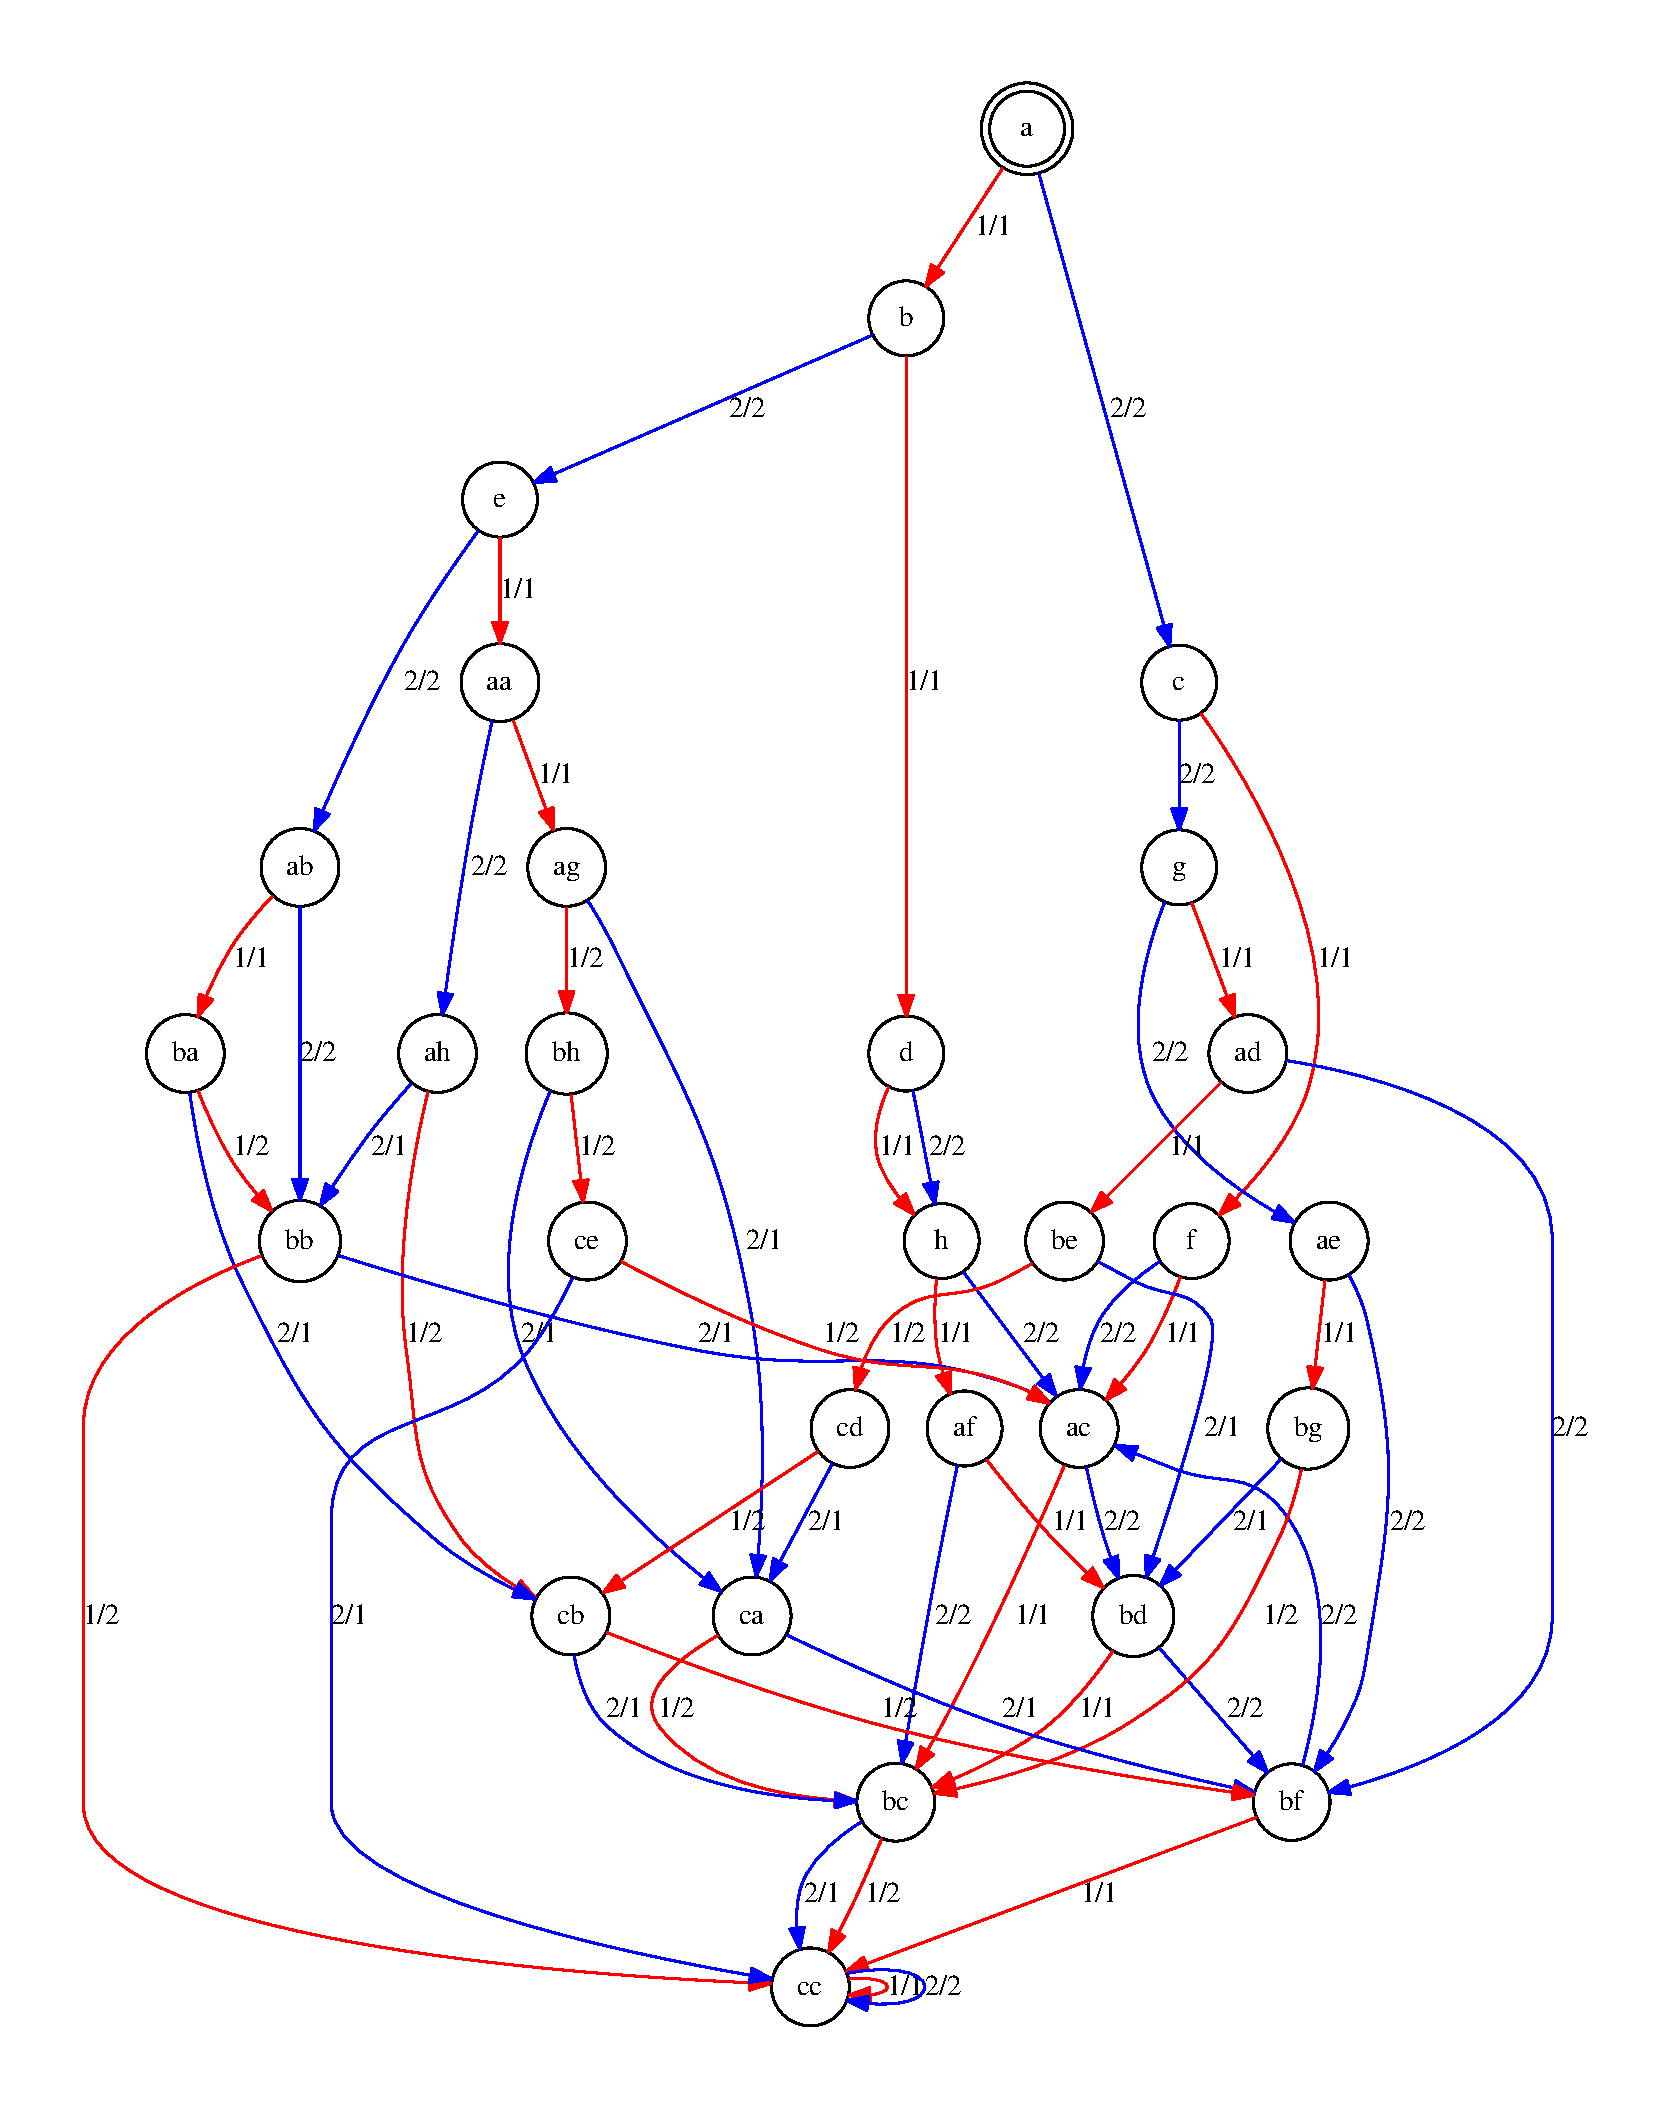
\includegraphics[width=\textwidth]{gap/PCD/noncomm29states}
 \caption{Element of the derived subgroup of the Grigorchuk group which is not a commutator.}\label{fig:noncomm}
\end{figure}
This finishes the proof of Theorem~\ref{thm:CWGrigorchukGroup}.
\subsection{Bounded conjugacy width}
In \cite{Fink:Conjugacy_growth} it is proven that $G$ has finite bounded conjugacy width. Here we give an explicit bound 
on this width.
\begin{pro}\label{pro:productOf6Conjugates}
 Let $g$ be in $G'$. Then the equation 
 \begin{align*}
  a^{X_1}a^{X_2}a^{X_3}a^{X_4}a^{X_5}ag=1
 \end{align*}
is solvable in $G$. 
\end{pro}
\begin{proof}
We need to solve the constrained equation $(\eq{E}=a^{X_1}a^{X_2}a^{X_3}a^{X_4}a^{X_5}ag,\gamma)$ for
some constraint $\gamma$. Independent of the chosen constraint the replacement of
the variable $X_i$ by $\pair{Y_i,Z_i}\act(\gamma(X_i))$ leads after normalization to an equivalent equation 
$R_2(g\at{2})(g\at{1})$. Similar to the construction of $\Gamma^q$ in the section
before one can find for each $q\in\RNK{G'}{K'}$ a constraint $\gamma$ such that
$\gamma(\eq{E}^{\id*\pi})=1$ and $\gamma'\in\Gamma_1(\gamma)$ such that for all 
$g\in\pi^{-1}(q)$ the pairs $(g\at{2}g\at{1},\gamma')$ are good pairs and $\gamma'$ is 
an active constraint.

Therefore the constrained equation $(R_2(g\at{2})(g\at{1}),\gamma')$ is solvable
by Corollary~\ref{cor:solvableConstraintedEquations}
for each $g\in G'$ and hence the equation $a^{X_1}a^{X_2}a^{X_3}a^{X_4}a^{X_5}ag$.

In GAP the function \gapinline{verifyExistGoodConjugacyConstraints} implements 
this condition.
\end{proof}	
\begin{lem}
 There exits an element $g\in G'$ such that the equation 
 \begin{align*}
  a^{X_1}a^{X_2}a^{X_3}ag=1
 \end{align*}
 is not solvable.
\end{lem}
\begin{proof}
As before independent of the activities of a possible constraint $\gamma$ and of the element $g\in G'$
the normalform of $\Phi_\gamma(a^{X_1}a^{X_2}a^{X_3}ag)$ turns out to
be $R_1(g\at{2}) g\at{1}$. So all there is to prove is that there is an element $h\in K$
where the products of states $h\at{2}\cdot h\at{1}$ is not a commutator.

The element $g$ displayed in Figure~\ref{fig:noncomm} provides such an element. It can easily be verified 
that $\pair{(cag)^\pi,(ac)^\pi}\in Q_1$ and $\omega(\pair{(cag)^\pi,(ac)^\pi})=1$. Thus by
the properties of the branch structure it is true that $\pair{(cag)^\pi,(ac)^\pi}\in K<G'$. 
\end{proof}
This finishes the proof of Corollary~\ref{cor:productOf6Conjugates}.
\begin{defi}[\cite{Fink:Conjugacy_growth}]
 The \emph{conjugacy width} of a group $G$ with respect to a generating set $S$ 
 is the smallest number $N\in\NN$ such that every element $g\in G$ is a product of
 at most $N$ conjugates of generators $s\in S$.
\end{defi}
\begin{cor}
 The Grigorchuk group $G$ with generating set $\{a,b,c,d\}$ has conjugacy width at most $8$.
\end{cor}
\begin{proof}
 The following set $T$ is a transversal of $\RNK{G}{G'}$. So every element $g\in G$ can be written as $g=th$ with $t\in T$ and $h\in G'$.
 \[T=\{1,a,d^aa,d^a,b,ab^a,ca^d,bd^a\}.\]
 As every element of $G'$ is a product of at most $6$ conjugates of $a$ this proofs the claim.
%  \begin{align}
%   T &=\{&1&,&a&,&ad=d^aa&,&ada=d^a,\\
%     & &b&,&ba=ab^a&,&bad=ca^d&,&bada=bd^a\}
%  \end{align}

\end{proof}

%no need for this any more!
% \begin{lem}
%  If $g\in K$ then 
%  \[(g\at{1},g\at{2})^{\pi\times\pi} \in \left\{\left(\left((ca)^n\right)^\pi,\left((ac)^n\right)^\pi\right) \mid n=1,\dotsc,4\right\}\]
% \end{lem}

\section{Proof of Theorem~\ref{thm:subgroups}}
We will proof the statement first for finite index subgroups. 
\begin{pro}\label{pro:f.i.subgroupsFiniteCW}
  All subgroups $H \leq G$ of finite index are of finite commutator width.
\end{pro}
\begin{proof}
 Note that from Corollary~\ref{cor:KhasCW2} it follows that $K\times K$ and furthermore 
 $K^{\times n}$ have commutator width $2$. 
 
 Let $H$ be a subgroup of finite index. Since $G$ has the congruence subgroup property
 (\cite{Bartholdi-Grigorchuk:parabolicSubgroups}) we can find a nontrivial normal subgroup $N=\Stab_G(m)<H$
 for some $m\in\NN$. Furthermore from the discussion of the top of the lattice of normal subgroups
 in $G$ done in \cite{Bartholdi-Grigorchuk:parabolicSubgroups} we can see that 
 \begin{align*}
  K&<\Stab_G(1), & K\times K&<\Stab_G(2), & K^{\times 4}&<\Stab_G(3).
 \end{align*}
 Furthermore it is $\Stab_G(n)=\Stab_G(3)^{\times 2^{n-3}}$ for $n\geq 4$ and hence for every 
 subgroup $H$ of finite index there is an $n$ such that $K^{\times 2^n}\leq H$.
  
  Since $G$ is just infinite, $[K^{\times2^n},K^{\times2^n}]$ has finite index in $[H,H]$.
  Taken a transversal $T$ of $\RNK{[H,H]}{[K^{\times2^n},K^{\times2^n}]}$ we can find 
  $m\in \NN$ such that every element in $T$ is a product of at most $m$ commutators in $H$.
  We can thus write each element $h\in [H,H]$ as product $kt$ with $k\in K^{\times 2^n}$, 
  $t\in T$ and thus as a product of at most $2+m$ commutators.  
\end{proof}
Now we can use that every infinite finitely generated subgroup of $G$ is 
abstractly commensurable with $G$ which can be seen in 
\cite[Theorem~1]{Grigorchuk-Wilson:Commensurability}.

This, by definition, means that every infinite finitely generated subgroup $H\leq G$ 
contains a finite index subgroup which is isomorphic to a finite index subgroup
of $G$ and hence by Proposition~\ref{pro:f.i.subgroupsFiniteCW} has finite
commutator width. This finishes the proof of the following proposition:
\begin{pro} \label{pro:fgsubgroupcw}
   All finitely generated subgroups $H \leq G$ are of finite commutator width.
\end{pro}
To show that there can't be a bound on the commutator width of subgroups
we need some results, which have
been established before. Since we couldn't find an original reference we will
sketch their proofs here.

\begin{pro}\ 
 \begin{enumerate}
  \item For all $n\in\NN$ there is a finite $2$-group of commutator width at least $n$.
  \item $K$ contains every finite $2$-group as a subgroup.
  \item Every finite $2$-group is a quotient of two finite index subgroups of $G$.
 \end{enumerate}
\end{pro}
\begin{proof}\
 \begin{enumerate}
  \item Consider the groups $\Gamma_n=\RNK{F_n}{\langle \gamma_3(F_n),x_1^2,\dotsc,x_n^2\rangle}$. 
  These are commutator extensions of $C_2^n$ by $C_2^{\binom{n}{2}}$ and are class $2$-nilpotent $2$-groups.
  The derived subgroup is hence of order $2^{\binom{n}{2}}$.
  Let $T$ be a transversal of $\RNK{\Gamma_n}{\Gamma_n'}$. Thus $T$ is of order $2^n$ and
  for $x,y\in\Gamma_n$ there are $t,s\in T$ and $x',y'\in\Gamma'$ such that
  every commutator $[x,y]=[tx',sy']=[t,s]$. Therefore there are at most $\binom{2^n}{2}$ commutators.
  
  This means there are at most $\binom{2^n}{2}^m\leq 2^{(2n-1)m}$ products of $m$ commutators 
  but the size of $\Gamma_n'$ is $2^{\binom{n}{2}} \geq2^{\frac{n^2}{4}}$ and hence 
  the commutator width of $\Gamma_{8m}$ is at least $m$.
  \item  $K$ contains for each $n$ the $n$-fold iterated wreath product
  $W_n(C_2)=C_2\wr \ldots \wr C_2$. 
  This can be found by finding finitely many vertices of the tree $T_2$ which
  are isomorphic to a finite binary rooted tree of $k$ levels $T_2^k$ and finding 
  elements $k_i\in K$ such that $\left<k_i\right>$ acts on $T_2^k$ like the full group of 
  automorphisms $\Aut(T_2^k)\simeq W_k(C_2)$.
  
  Then 
  since $W_n(C_2)$ is a Sylow $2$-subgroup of $S_{2^n}$ every finite $2$-group is a subgroup of
  $W_n(C_2)$ for some $n$ and hence of $K$.
  \item Consider again the vertices of $T_2$ which are isomorphic to a
  the finite tree $T_2^k$ on which a subgroup of $K$ acts like $W_n(C_2)$. If we take $m$ large
  enough such that all this vertices are above the $m$-th level we can find a copy of $W_n(C_2)$
  inside $\RNK{G}{\Stab(m)}$.
 \end{enumerate}
\end{proof}
In the following theorem we summarize our results for the commutator width of the Grigorchuk Group.
\begin{thm}\ 
 \begin{enumerate}
  \item $G$ and its branching subgroup $K$ have commutator width $2$. \label{thm:summeryStat1}
  \item All finitely generated subgroups $H\leq G$ have finite commutator width.\label{thm:summeryStat2}
  \item \label{thm:summeryStat3} The commutator width of subgroups is unbounded even among finite index subgroups.
  %\item There exists subgroups with infinite commutator width.\label{thm:summeryStat4}
 \end{enumerate}
\end{thm}
\begin{proof}
 Statements~(\ref{thm:summeryStat1}) and (\ref{thm:summeryStat2}) are proven in Theorem~\ref{thm:CWGrigorchukGroup} and Proposition~\ref{pro:fgsubgroupcw}.
 %Since $G$ contains every finite $2$ group as a subgroup there are subgroups of arbitrary large commutator width. 
 %The restricted product
 %of these groups is a subgroup of the restricted product of infinite copies of $K$ and since $K^n\leq K$ for all $n$ this inverse limit is a subgroup of $G$.
 %TODO: this inverse limit is a subgroup of $G$. No it isn't ?!?
 For every $n\in\NN$ we can find two groups $H_1,H_2$ of finite index in $G$ such that $\RNK{H_1}{H_2}$ has commutator
 width at least $n$. Then $H_1$ has commutator width at least $n$ as well and thus the commutator width of finite index subgroups can not be bounded.
\end{proof}
\section{Implementation in GAP}
\subsection{Usage of the attached files} \label{sec:gap_verify}
In the main directory of the archive one can type the command \gapinline{gap verify.g} and 
will get as output a list of functions with their return value. All these functions should
return \gapinline{true}. 

This approach uses precomputed data which are also in the archive. This saves a lot of
computation time.

However this data can be recomputed if a sufficiently new version of GAP and
some packages are present. For details see Section \ref{sec:precomputation}.

This is what the functions check:
\begin{description}
\item[\texttt{verifyLemma90orbits}] This function verifies that there are
  indeed $90$ orbits of $\RNK{Q^6}{\Stab(R_3}$ as claimed in Lemma~\ref{lem:90Constraints}. 
\item[\texttt{verifyLemma86orbits}] Analogously to the previous function 
  this one verifies that there are $86$ orbits of $\RNK{Q^4}{\Stab(R_2)}$. 
\item[\texttt{verifyLemmaExistGoodConstraints}] This verifies that for each 
  $q\in\RNK{G'}{K'}$ there is some $\gamma\in\Red_{act}$ such that $(q,\gamma)$ 
  forms a good pair. This is claimed in Lemma~\ref{lem:existsGoodGamma}.
\item[\texttt{verifyLemmaExistGoodConstraints4}] This is the sharper version
  of the function before. It checks that the above statement is already true 
  if one replaces $\Red_{act}$ by $\Red_{act}^4$ as claimed in 
  Lemma~\ref{lem:existsGoodGammaForRed4}.
\item[\texttt{verifyPropExistsSuccessor}] This verifies that for
  each good pair $(q,\gamma) \in\RNK{G'}{K'}\times(\Red_{act}\cup \Red_{act}^4)$ there exists 
  a $\gamma'\in\Gamma^q(\gamma)$ such that all preimages of 
  $\bar p_{\textup{rep}(Y_{\gamma'})}(q)$ under the map $\rho'$ form
  good pairs with the constraint $\gamma'$. This is needed in the proof of
  Proposition~\ref{pro:existsNextPair} and Proposition~\ref{pro:existsNextPair4}.
\item[\texttt{verifyCorollaryFiniteCWK}] Corollary~\ref{cor:KhasCW2} needs the
  existence of succeeding good pairs of the pair $(1,\id)\in\RNK{K'}{K'}\times\Red^4$.
  This function verifies this existence. 
\item[\texttt{verifyExistGoodConjugacyConstraints}] This verifies that for the equation
  $a^{X_1}a^{X_2}a^{X_3}a^{X_4}a^{X_5}a$ there are constraints $\gamma$ 
  that inherit good succeeding pairs. This is needed in the proof of
  Proposition~\ref{pro:productOf6Conjugates}.
\item[\texttt{verifyGermGroup4hasCW}] This function verifies the existence of 
  an element in the derived subgroup of the $4$-th level germgroup that is not a commutator.
\end{description}

\subsection{Precomputed data}\label{sec:precomputation}
In the interactive gap shell started by \gapinline{gap verify.g}
the precomputed data is read from some files in \filename{gap/PCD/} and stored in 
a record \gapinline{PCD}. 

One can use the function \gapinline{RedoPrecomputation} with one argument. In each case
the result is written to one ore multiple files and will override the original precomputed data. 
The argument is a string and can be one of the following:
\begin{description}
    \item [\texttt{``orbits''}] This will compute the $90$ orbits of $\RNK{\Aut(F_6)}{\Stab(R_3)}$ and the
		       $86$ orbits of $\RNK{\Aut(F_4)}{\Stab(R_2)}$. This computation will take
		       about $12$ hours on an ordinary machine and has no progress bar.
   \item [\texttt{``goodpairs''}] First this will compute for each constraint $\gamma\in\Red\cup\Red^4$ 
		      the set of all $q\in\RNK{G'}{K'}$ such that $(q,\gamma)$ is a good pair.
		      
		      Then it computes for each good pair $(q,\gamma)$ one $\gamma'\in\Gamma_q(\gamma)$
		      with decorated $X=Y_{\gamma'}\in S$ as defined in equation~\ref{def:Gammaq} which 
		      fulfills depending whether $\gamma\in\Red^4_{act}$ or $\gamma\in\Red_{act}$ 
		      either Proposition~\ref{pro:existsNextPair} or Proposition~\ref{pro:existsNextPair4}.
		      This computation will take about $2$ hours on ordinary machines and is equipped 
		      with a progress bar. 
		      
		      Afterwards the succeeding pairs of $(1,\id)$ are computed which are needed for 
		      Corollary~\ref{cor:KhasCW2}. 
   \item [\texttt{``conjugacywidth''}] Denote by $\eq{E}_g$ the equation $a^{X_1}a^{X_2}a^{X_3}a^{X_4}a^{X_5}ag$.
		      For each $g^\tau=q\in\RNK{G'}{K'}$ this will compute a constraint 
		      $\gamma\colon F_5 \to Q$ for the equations $\eq{E}_g$
		      and a constraint $\gamma'\colon F_4\to Q$ such that
		      $(\gamma * \pi)(\eq{E}_g) = 1$,
		      \[\eq{E}'_g := \nf(\Phi_\gamma(\eq{E}_g))=[X_1,X_2][X_3,X_4](g\at{2})(g\at{1}),\] and
		      $(\eq{E}'_g,\gamma')$ is a good pair for all $g$ with $g^\tau=q$.
		      
		      The computation will take about one hour and is equipped with a progress bar.
   \item [\texttt{``charactertable''}] This will compute the character table of the $4$-th level germgroup
		      and the set of irreducible characters. 
		      As the germgroup is quite large, this
		      will take about $3$ hours. There is no kind of progress bar.
   \item [\texttt{``noncommutator''}] Inside the $4$-th level germgroup there is an element which is not
		      a commutator but in the commutator subgroup. This command will find this 
		      element using the character table of the germgroup. The search will be 
		      almost immediately give a result. Most of the computation time is used
		      to assert that the found element is indeed not a commutator.
		      
		      The element is then used to compute a preimage in $G$ with a minimal 
		      number of states.

		      Checking the assertion will take approximately $3$ hours and is equipped 
		      with a progress bar. 
  \item [\texttt{``all''}] This will do all of the above one after another.		      
   \end{description}
To recompute the orbits or the charactertable GAP should be 
started with the \gapinline{-o} flag
to provide enough memory for the computation. For example start GAP by 
\gapinline{gap -o 8G verify.g}


\subsection{Implementation details}
\label{sec:gap_details}
\subsubsection{Reduced Constraints}
The proof of Lemma~\ref{lem:finitelyManyConstraints} in \cite{Lysenok-Miasnikov-Ushakov:QuadraticEquationsInGrig} 
provides a constructive method to reduce any constraint to one with support
only in the first five variables. 
We have implemented this in the function \gapinline{ReducedConstraintAllModes} in the file
\filename{gap/functions.g}.

It uses that the quotient $Q=\RNK{G}{K}$ is a polycyclic group with 
\begin{align*}
 C_0 &= Q = \left<a^\pi,b^\pi,d^\pi\right>, &
 C_1 &= \left<a^\pi,d^\pi\right>, &
 C_2 &= \left<(ad)^\pi\right>.
\end{align*}
We take the generators of $\Stab(R_n)$ as given in the proof of Lemma~\ref{lem:90Constraints}
plus additional ones which can switch two neighboring pairs:
\begin{align*}
 s_i &\colon &X_i&\mapsto X_{i+2}&\\
	    &&X_i+1&\mapsto X_{i+3}&\\
	    &&X_i+2&\mapsto X_{i}^{[X_{i+2},X_{i+3}]}&\\
	    &&X_i+3&\mapsto X_{i+1}^{[X_{i+2},X_{i+3}]} & \textup{ for }i = 1,3,\dotsc,2n-3.
\end{align*}
It can easily be checked, that these are also contained in $\Stab(R_n)$. These elements
are used to reduce a given constraint in a form of a list with entries in $Q$ to a
list where all entries with index larger then $5$ are trivial. 
This constraint can then be further reduced by a lookup table for the orbits
of $\RNK{\Aut(F_6)}{\Stab(R_3)}$. 

If the file \filename{verify.g} is loaded in a GAP environment with the FR package available 
the function \gapinline{ReducedConstraint} can be used as an alias to get 
reduced constraints. For Example:
 \begin{lstlisting}
    gap> f1 := Q.3;
    gap> gamma:= [f1,f1,f1,f1,f1,f1];
    gap> constr := ReducedConstraint(gamma);;
    gap> Print(constr.constraint);
\end{lstlisting} 
\begin{verbatim}
[ <id>, <id>, <id>, <id> , f4, <id>]
\end{verbatim} 

\subsubsection{Good pairs}
For $g\in G$ and a constraint $\gamma$ the question if $(g,\gamma)$ is a good
pair depends only on the image $g^\tau\in\RNK{G}{K'}$ and the representative
of $\gamma\in\Red$. (See Section~\ref{sec:good_pairs}.) So this is already a
finite problem. 

For a given constraint $\gamma$ to get all $q$ which form a good pair we can
enumerate all possible commutators for $r_i\in\rho^{-1}(\gamma(X_i))$.
$[r_1,r_2][r_3,r_4][r_5,r_6]$. Since $\lvert\RNK{K}{K'}\rvert=64$ considering all 
combinations at once is far from beeing efficient thus the possible values for
$[r_1,r_2]$ are computed and in a second step products of those elements.
This is implemented in the function \gapinline{goodPairs} in the file
\filename{gap/functions.g}.
\subsubsection{Successors}
The key ingredient for the proof of Theorem~\ref{thm:CWGrigorchukGroup} is
Proposition~\ref{pro:existsNextPair}. The computational effort there is
to compute the sets $\Gamma_q(\gamma)$ and find good pairs inside of them.

This is implemented exactly as explained in the construction of the map
$\Gamma_q$ in the function \gapinline{GetSuccessor} in the file 
\filename{gap/precomputeGoodPairs.g}. Given an element $q\in\RNK{G'}{K'}$ 
and an active constraint $\gamma$ this function returns a tuple $(\gamma',X)$ 
with $\gamma\in\Red$ and $X$ the decorated element $Y_\gamma'$.

Given an inactive constraint $\gamma$ it returns a pair of constraints
$\gamma_1,\gamma_2$ such that both have nontrivial activity and with
$\omega$ the map from the branch structure it holds:
$\omega(\pair{\gamma_1(X_i),\gamma_2(X_i)})=\gamma(X_i)$. 

If the FR package is available
the function \gapinline{GetSuccessorLookup} can be used to explore the
successors of elements. It returns the succeeding pair. For example
 \begin{lstlisting}
    gap> f4 := Q.1;
    gap> gamma:= [f4,f4,f4,f4,f4,f4];;
    gap> g := (a*b)^8;;
    gap> IsGoodPair(g,gamma);
\end{lstlisting}
\begin{verbatim}
true
\end{verbatim} 
\begin{lstlisting}
    gap> suc := GetSuccessorLookup(g,gamma);;    
    gap> suc[1];
\end{lstlisting}
\begin{verbatim}
<Trivial Mealy element on alphabet [ 1 .. 2 ]>
\end{verbatim} 
\begin{lstlisting}
    gap> suc[2].constraint;
\end{lstlisting}
\begin{verbatim}
[ <id>, <id>, <id>, <id>, f1*f3, <id> ]
\end{verbatim} 



%\paragraph{Lemma~\ref{lem:atIsWellDefinedModK'}}
%\paragraph{Lemma~\ref{lem:existsGoodGamma}}

\bibliography{latex/bio}
\appendix
% \include{Abschnitte/Anhang}
%\include{Abschnitte/Erklaerung}


\end{document}
